\chapter{随机向量与联合分布}
\label{chap:random-vectors}
\label{chap:probability-theory}

第~\ref{chap:random-variables}章每次只研究一个随机变量。实际问题却常常同时记录几个量：同一位学生考前的复习次数与考试是否通过，两台传感器对同一温度的读数，一批多分类试验中各类别出现的次数。分别写出每个量的分布，仍回答不了“两个量是否倾向于一起偏高”“知道其中一个以后，另一个的可能性怎样改变”“它们的和服从什么分布”这类问题，因为这些问题都涉及几个量在同一次试验中的共同取值。

本章研究多个随机变量的共同描述。前四节先建立联合分布、边缘分布和联合数值特征，再分别讨论独立关系与条件关系：独立表示一个变量不提供关于另一个变量的信息，条件分布则说明获得信息以后怎样重新计算概率。第五、六节方向相反：前者从已知分布出发，计算和、比值、仿射变换等组合量的分布；后者从目标分布出发，寻找能够产生它的随机输入和操作。最后一节把这些操作集中用于多元高斯分布，在一个模型里完成生成、边缘化、独立判定和条件计算。

本章沿用第~\ref{chap:random-variables}章的范围：只处理由质量函数求和或由普通密度积分计算概率的模型。多元积分、换元公式和矩阵分解分别取自第~\ref{chap:multivariate-integration}章与前面的矩阵各章。更一般的联合分布和条件分布需要测度论，可参考\BookPartRef{part:probability-spaces}{卷2《数学准备：抽象数学》的“概率空间”部分}。

\section{随机向量与联合分布}
\label{sec:rvec-joint}

研究几个量的共同取值，首先要把它们放在同一次试验里，并给“几个量同时满足某些条件”这类事件赋予概率。本节先建立这一描述，再说明怎样从中取出单个分量的分布，以及为什么反过来不行。

\subsection{随机向量与联合分布}

\paragraph{随机向量}
设$X$表示一名学生考前一周复习的次数，$Y$表示他的考试是否通过（通过记为$1$）。分别知道$X$和$Y$的分布，只能回答“复习两次的学生占多少”“通过的学生占多少”；要问“复习两次且通过的学生占多少”，就必须知道两个量在同一名学生身上怎样同时取值。

\begin{definition}[随机向量与联合分布]
设$X_1,\ldots,X_d$是定义在同一随机试验上的随机变量。把它们排成列向量
\[
 \bm X=(X_1,\ldots,X_d)^{\top},
\]
称为$d$维\term{随机向量}（random vector）。试验每进行一次，$\bm X$得到一个实现值$\bm x\in\mathbb R^d$。对$\mathbb R^d$中的集合$A$，$\{\bm X\in A\}$是一个事件；这些事件的概率$\mathbb P(\bm X\in A)$合起来称为$\bm X$的\term{联合分布}（joint distribution）。
\end{definition}

“同一随机试验”这一条件不可省略。只有当$X$和$Y$描述同一名学生、同一次测量或同一批试验时，$\{X=2,Y=1\}$才是一个有意义的事件。随机向量本身仍是随机量，实现值$\bm x$是一次观测得到的普通向量；与第~\ref{chap:random-variables}章一样，我们用大写字母表示前者，用小写字母表示后者。

\paragraph{离散情形：二维概率表}
若$X$与$Y$都只取有限个或可数个值，联合分布由
\[
 p_{X,Y}(x,y)=\mathbb P(X=x,\,Y=y)
\]
完全确定，称为\term{联合质量函数}（joint probability mass function）。它非负，对全部取值求和等于$1$；任意事件的概率等于事件所含取值对的质量之和：
\[
 \mathbb P\bigl((X,Y)\in A\bigr)=\sum_{(x,y)\in A}p_{X,Y}(x,y).
\]
两个变量各取有限个值时，联合质量函数就是一张二维概率表。

\begin{example}[复习次数与考试结果]
\label{ex:rvec-study-table}
作为教学示例，设复习次数$X\in\{0,1,2\}$与考试结果$Y\in\{0,1\}$的联合概率如图~\ref{fig:rvec-joint-table}(a)左侧的六个格子所示。复习至少一次且通过的概率是
\[
 \mathbb P(X\ge1,\,Y=1)=p_{X,Y}(1,1)+p_{X,Y}(2,1)=0.25+0.25=0.50.
\]
事件$\{X>Y\}$包含取值对$(1,0)$、$(2,0)$与$(2,1)$，故$\mathbb P(X>Y)=0.15+0.05+0.25=0.45$。计算任何联合事件，都只需在表中圈出相应格子并相加。
\end{example}

\begin{figure}[htbp]
  \centering
  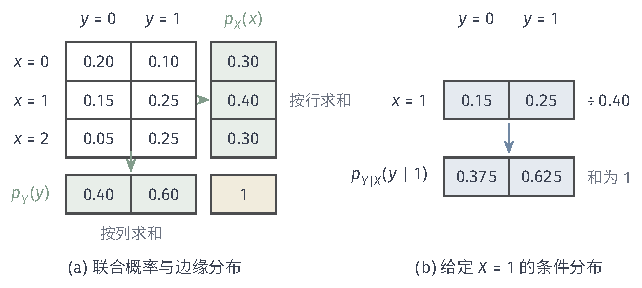
\includegraphics[width=108.8mm]{figures/01-basic-mathematics/05-probability-and-statistics-basics/tikz/rvec-joint-table/figure.pdf}
  \caption{二维概率表。(a)中白色格子是复习次数$X$与考试结果$Y$的联合概率，六个数之和为$1$；按行求和得到右侧$X$的边缘分布，按列求和得到下方$Y$的边缘分布。(b)取出$X=1$一行，除以该行之和$0.40$，得到给定$X=1$时$Y$的条件分布。}
  \label{fig:rvec-joint-table}
\end{figure}

\paragraph{连续情形：联合密度}
若$(X,Y)$的取值连续变化，单个点的概率为零，需要像一元情形那样用密度累计概率。称非负函数$f_{X,Y}$为$(X,Y)$的\term{联合密度}（joint density），如果对平面上的矩形以及第~\ref{chap:multivariate-integration}章能够积分的区域$A$，都有
\[
 \mathbb P\bigl((X,Y)\in A\bigr)=\iint_A f_{X,Y}(x,y)\,\mathrm dx\,\mathrm dy .
\]
取$A=\mathbb R^2$可知联合密度的积分为$1$。与一元情形相同，$f_{X,Y}(x,y)$本身不是概率；在$(x,y)$附近边长为$h,k$的小矩形上，概率约为$f_{X,Y}(x,y)hk$，所以联合密度表示单位面积上的概率。$d$维情形把二重积分换成$d$重积分即可。

\begin{example}[正方形上的联合密度]
\label{ex:rvec-square-density}
令$f_{X,Y}(x,y)=x+y$，$0\le x,y\le1$，其余位置为零。先检查归一化：
\[
 \int_0^1\!\!\int_0^1(x+y)\,\mathrm dy\,\mathrm dx=\int_0^1\Bigl(x+\frac12\Bigr)\mathrm dx=1 .
\]
两个分量都不超过$1/2$的概率为$\int_0^{1/2}\!\int_0^{1/2}(x+y)\,\mathrm dy\,\mathrm dx=1/8$。事件$\{X+Y\le1\}$对应三角形区域，按累次积分计算：
\[
 \mathbb P(X+Y\le1)=\int_0^1\!\!\int_0^{1-x}(x+y)\,\mathrm dy\,\mathrm dx
 =\int_0^1\frac{(1-x)(1+x)}2\,\mathrm dx=\frac13 .
\]
密度在右上角较大，所以落在左下三角形的概率小于面积比$1/2$。本章后面会多次回到这个例子。
\end{example}

\paragraph{联合分布函数}
质量函数和密度分别适用于两类模型。与一元情形一样，分布函数给出不依赖模型类型的统一描述。对$d$维随机向量定义\term{联合分布函数}（joint distribution function）
\[
 F_{\bm X}(\bm x)=\mathbb P(X_1\le x_1,\ldots,X_d\le x_d),\qquad \bm x\in\mathbb R^d .
\]
二维时，矩形概率可以由四个角上的值算出。对$a_1<b_1$、$a_2<b_2$，事件$\{X\le b_1,Y\le b_2\}$去掉$\{X\le a_1,Y\le b_2\}$和$\{X\le b_1,Y\le a_2\}$，两者的公共部分$\{X\le a_1,Y\le a_2\}$被去掉了两次，需要加回一次，于是
\[
\begin{aligned}
 &\mathbb P(a_1<X\le b_1,\,a_2<Y\le b_2)\\
 &\quad=F_{X,Y}(b_1,b_2)-F_{X,Y}(a_1,b_2)-F_{X,Y}(b_1,a_2)+F_{X,Y}(a_1,a_2).
\end{aligned}
\]
所有矩形的概率确定以后，整个联合分布也就确定了；这一结论的一般证明留到卷二。对示例~\ref{ex:rvec-square-density}，在单位正方形内
$F_{X,Y}(x,y)=\int_0^x\!\int_0^y(s+t)\,\mathrm dt\,\mathrm ds=xy(x+y)/2$，代入$x=y=1/2$又得到$1/8$。

\paragraph{多项分布}
多次类别试验的计数向量是联合质量函数的典型例子。设一次试验的结果落入$K$个类别之一，类别$k$的概率为$\pi_k$，概率向量$\bm\pi=(\pi_1,\ldots,\pi_K)^{\top}$各分量非负且和为$1$。把试验独立重复$n$次，记$N_k$为结果落入类别$k$的次数，得到计数向量$\bm N=(N_1,\ldots,N_K)^{\top}$。

给定非负整数$n_1,\ldots,n_K$且$n_1+\cdots+n_K=n$。任取一个恰有$n_k$次落入类别$k$的具体结果序列，由试验的独立性，它的概率是$\pi_1^{n_1}\cdots\pi_K^{n_K}$。这样的序列共有$n!/(n_1!\cdots n_K!)$个，即把$n$个位置分成大小为$n_1,\ldots,n_K$的$K$组的方法数（第~\ref{chap:counting}章）。各序列互斥，把概率相加就得到下面的分布。

\begin{definition}[多项分布]
称$\bm N$服从参数为$n$与$\bm\pi$的\term{多项分布}（multinomial distribution），记为$\bm N\sim\operatorname{Mult}(n,\bm\pi)$，若
\[
 \mathbb P(N_1=n_1,\ldots,N_K=n_K)=\frac{n!}{n_1!\cdots n_K!}\,\pi_1^{n_1}\cdots\pi_K^{n_K},
\]
其中$n_1,\ldots,n_K$为非负整数且$n_1+\cdots+n_K=n$；其他取值的概率为零。
\end{definition}

各分量之和恒等于$n$，这是多项分布最重要的结构：$\bm N$的取值只落在满足$\sum_kn_k=n$的整数点上。$K=2$时，$N_1$就是$n$次试验中“落入第一类”的次数，服从$\operatorname{Bin}(n,\pi_1)$，而$N_2=n-N_1$完全由$N_1$决定。

\begin{example}[三类结果的计数]
\label{ex:rvec-multinomial}
设$n=4$，$\bm\pi=(0.5,0.3,0.2)^{\top}$。恰好两次落入第一类、第二类和第三类各一次的概率为
\[
 \mathbb P\bigl(\bm N=(2,1,1)^{\top}\bigr)=\frac{4!}{2!\,1!\,1!}\,0.5^2\times0.3\times0.2=12\times0.015=0.18 .
\]
而$\mathbb P\bigl(\bm N=(2,2,1)^{\top}\bigr)=0$，因为$2+2+1\neq4$。
\end{example}

\subsection{边缘分布}

\paragraph{从联合分布求边缘分布}
有了联合分布，常常又只关心其中一部分分量，例如只问复习次数$X$本身的分布。事件$\{X=x\}$可以按$Y$的取值拆成互斥事件$\{X=x,Y=y\}$之并，由可加性，
\[
 p_X(x)=\sum_y p_{X,Y}(x,y),\qquad p_Y(y)=\sum_x p_{X,Y}(x,y).
\]
这就是二维概率表按行或按列求和。具有联合密度时，取$A=[a,b]\times\mathbb R$，并按第~\ref{chap:multivariate-integration}章的累次积分先对$y$积分（被积函数非负，无穷区间上的积分按截断取极限理解），得到
\[
 \mathbb P(a\le X\le b)=\int_a^b\Bigl(\int_{-\infty}^{\infty}f_{X,Y}(x,y)\,\mathrm dy\Bigr)\mathrm dx ,
\]
所以$f_X(x)=\int f_{X,Y}(x,y)\,\mathrm dy$是$X$的密度。这样得到的单个分量的分布称为\term{边缘分布}（marginal distribution），对其余分量求和或积分的操作称为\term{边缘化}（marginalization）。高维时同理：保留哪些分量，就对其余全部分量求和或积分。

图~\ref{fig:rvec-joint-table}(a)中，按行求和得到$p_X=(0.30,0.40,0.30)$，按列求和得到$p_Y=(0.40,0.60)$。示例~\ref{ex:rvec-square-density}中，$f_X(x)=\int_0^1(x+y)\,\mathrm dy=x+1/2$，$0\le x\le1$；由对称性，$f_Y(y)=y+1/2$。对多项分布，只看第$k$类是否出现，每次试验以概率$\pi_k$“成功”且各次独立，所以边缘分布是$N_k\sim\operatorname{Bin}(n,\pi_k)$。

\paragraph{边缘分布不能确定联合分布}
边缘化把其他分量的信息汇总掉，这一步一般不能逆转。设$X$与$Y$都等可能取$0$或$1$。第一种联合分布让四个取值对各有概率$1/4$；第二种只允许$(0,0)$与$(1,1)$，各有概率$1/2$，即$Y=X$。两张表按行、按列求和都得到$(1/2,1/2)$，边缘完全相同；但前者$\mathbb P(X=Y)=1/2$，后者$\mathbb P(X=Y)=1$。

\begin{example}[随机变号]
\label{ex:rvec-random-sign}
令$Z\sim\mathcal N(0,1)$，$S$与$Z$独立，等可能取$1$或$-1$，再令$X=Z$，$Y=SZ$。由$Z$的对称性，
\[
 \mathbb P(Y\le y)=\tfrac12\mathbb P(Z\le y)+\tfrac12\mathbb P(-Z\le y)=\Phi(y),
\]
其中$\Phi$是标准高斯分布函数，所以$Y$也服从$\mathcal N(0,1)$。图~\ref{fig:rvec-same-marginals}比较了它与两个独立标准高斯变量：上方和右侧的边缘直方图几乎一样，散点却截然不同。随机变号的散点全部落在两条对角线$|y|=|x|$上，知道$X$以后$Y$只剩两个可能值。
\end{example}

\begin{figure}[htbp]
  \centering
  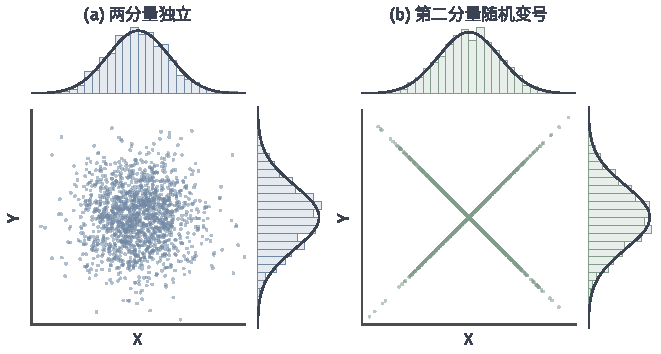
\includegraphics[width=112mm]{figures/01-basic-mathematics/05-probability-and-statistics-basics/matplotlib/rvec-same-marginals/figure.pdf}
  \caption{边缘分布相同、联合分布不同。两幅图各有$1500$个模拟点（固定随机种子）：(a)中$X,Y$是独立的标准高斯变量；(b)中$X=Z$，$Y=SZ$，$S$等可能取$\pm1$并与$Z$独立。两图上方与右侧的直方图都与标准高斯密度（黑线）吻合，但(b)的全部点落在两条对角线上。}
  \label{fig:rvec-same-marginals}
\end{figure}

因此，单独知道每个分量的分布还不足以回答涉及几个分量的问题。联合分布在边缘分布之外还记录了分量之间的联系；后面三节分别从数值特征、独立性和条件分布三个角度描述这种联系。

\section{联合分布的数值特征}
\label{sec:rvec-moments}

完整的联合分布包含很多信息，在高维时尤其难以直接列出或画出。第~\ref{chap:random-variables}章用期望和方差概括单个分布的位置与波动；对随机向量，我们还需要一个量来概括分量之间怎样一起变化。

\subsection{均值向量}

\paragraph{定义与线性性}
随机向量的中心位置可以逐个分量描述。设每个分量都有有限期望，即$\mathbb E|X_i|<\infty$，定义\term{均值向量}（mean vector）
\[
 \bm\mu=\mathbb E\bm X=(\mathbb EX_1,\ldots,\mathbb EX_d)^{\top}.
\]
每个$\mathbb EX_i$只依赖$X_i$的边缘分布，也可以直接对联合分布计算：与一元情形相同，函数$g(\bm X)$的期望按
\[
 \mathbb E\,g(\bm X)=\sum_{\bm x}g(\bm x)p_{\bm X}(\bm x)
 \quad\text{或}\quad
 \mathbb E\,g(\bm X)=\int_{\mathbb R^d}g(\bm x)f_{\bm X}(\bm x)\,\mathrm d\bm x
\]
计算，只要求和或积分绝对收敛，无须先求出$g(\bm X)$的分布。取$g(x,y)=x+y$，把求和拆成两项，
\[
 \mathbb E(X+Y)=\sum_{x,y}x\,p_{X,Y}(x,y)+\sum_{x,y}y\,p_{X,Y}(x,y)=\mathbb EX+\mathbb EY .
\]
积分情形相同。由此，对常向量$\bm a$、常数$b$以及$m\times d$常矩阵$\bm A$、常向量$\bm b$，
\[
 \mathbb E(\bm a^{\top}\bm X+b)=\bm a^{\top}\bm\mu+b,\qquad
 \mathbb E(\bm A\bm X+\bm b)=\bm A\bm\mu+\bm b .
\]
第二式逐行使用第一式即得。这些等式不需要分量之间有任何独立性。

\paragraph{均值只描述中心}
示例~\ref{ex:rvec-study-table}中$\mathbb EX=0\times0.3+1\times0.4+2\times0.3=1$，$\mathbb EY=0.6$，故$\bm\mu=(1,0.6)^{\top}$；示例~\ref{ex:rvec-square-density}中$\mathbb EX=\int_0^1x(x+1/2)\,\mathrm dx=7/12$，由对称性$\bm\mu=(7/12,7/12)^{\top}$。

均值向量给出共同的中心位置，却没有说明分量怎样一起变化。回到上一小节两个边缘相同的二元例子：两种联合分布的均值向量都是$(1/2,1/2)^{\top}$。但在独立的那张表中，$X+Y$以概率$1/4,1/2,1/4$取$0,1,2$，方差为$1/2$；在$Y=X$的那张表中，$X+Y$等可能取$0$或$2$，方差为$1$。两个读数同时偏高或同时偏低时，和的波动更大，这需要一个新的数值特征来描述。

\subsection{协方差与相关系数}

\paragraph{协方差}
把和的方差展开，就能看出缺少的是哪一项。记$\mu_X=\mathbb EX$，$\mu_Y=\mathbb EY$，则
\[
\begin{aligned}
 \operatorname{Var}(X+Y)&=\mathbb E\bigl[(X-\mu_X)+(Y-\mu_Y)\bigr]^2\\
 &=\operatorname{Var}(X)+\operatorname{Var}(Y)+2\,\mathbb E\bigl[(X-\mu_X)(Y-\mu_Y)\bigr].
\end{aligned}
\]
前两项只依赖边缘分布，最后一项则依赖联合分布。

\begin{definition}[协方差]
设$\mathbb EX^2<\infty$，$\mathbb EY^2<\infty$。称
\[
 \operatorname{Cov}(X,Y)=\mathbb E\bigl[(X-\mu_X)(Y-\mu_Y)\bigr]
\]
为$X$与$Y$的\term{协方差}（covariance）。
\end{definition}

有限二阶矩保证这个期望有限：由$|uv|\le(u^2+v^2)/2$，中心化乘积的绝对值被两个平方项控制。展开乘积并用期望的线性性，得到常用的计算公式
\[
 \operatorname{Cov}(X,Y)=\mathbb E[XY]-\mu_X\mu_Y .
\]
中心化乘积$(X-\mu_X)(Y-\mu_Y)$在两个变量同时高于或同时低于各自均值时为正，一高一低时为负。协方差为正，表示“同向偏离”在概率加权下占优势；为负则表示“反向偏离”占优势。

协方差对每个变量都是线性的，并且不受平移影响：$\operatorname{Cov}(aX+b,cY+e)=ac\operatorname{Cov}(X,Y)$，$\operatorname{Cov}(X_1+X_2,Y)=\operatorname{Cov}(X_1,Y)+\operatorname{Cov}(X_2,Y)$；还有$\operatorname{Cov}(X,X)=\operatorname{Var}(X)$。于是开头的展开式推广为
\begin{equation}
 \operatorname{Var}(aX+bY)=a^2\operatorname{Var}(X)+b^2\operatorname{Var}(Y)+2ab\operatorname{Cov}(X,Y).
 \label{eq:rvec-variance-of-combination}
\end{equation}

\begin{example}[概率表中的协方差]
\label{ex:rvec-table-covariance}
对示例~\ref{ex:rvec-study-table}，$XY$只在$(1,1)$与$(2,1)$处非零，
\[
 \mathbb E[XY]=1\times0.25+2\times0.25=0.75,\qquad
 \operatorname{Cov}(X,Y)=0.75-0.6=0.15,
\]
复习次数多与考试通过倾向于同时出现。对上一小节$Y=X$的二元例子，$\operatorname{Cov}(X,Y)=\operatorname{Var}(X)=1/4$，代入式~\eqref{eq:rvec-variance-of-combination}得$\operatorname{Var}(X+Y)=1/4+1/4+2\times1/4=1$，与直接计算一致。
\end{example}

\paragraph{相关系数}
协方差的数值依赖单位：把$X$由米改成厘米，协方差扩大$100$倍，而两个量的联系并没有改变。用两个标准差$\sigma_X,\sigma_Y$去除，就得到与单位无关的量。

\begin{definition}[相关系数]
设$0<\operatorname{Var}(X)<\infty$，$0<\operatorname{Var}(Y)<\infty$。称
\[
 \operatorname{Corr}(X,Y)=\frac{\operatorname{Cov}(X,Y)}{\sigma_X\sigma_Y}
\]
为$X$与$Y$的\term{相关系数}（correlation coefficient），常记为$\rho_{X,Y}$或$\rho$。
\end{definition}

\begin{theorem}[相关系数的范围]
\label{thm:rvec-correlation-bound}
在上述条件下，$-1\le\rho_{X,Y}\le1$。并且$|\rho_{X,Y}|=1$当且仅当存在常数$a$与$b\neq0$，使$Y=a+bX$以概率$1$成立，此时$b$与$\rho_{X,Y}$同号。
\end{theorem}

\begin{proof}
令$U=(X-\mu_X)/\sigma_X$，$V=(Y-\mu_Y)/\sigma_Y$为两个标准化变量，则$\mathbb EU^2=\mathbb EV^2=1$，$\mathbb E[UV]=\rho$。对平方的期望展开，
\[
 0\le\mathbb E(V-\rho U)^2=\mathbb EV^2-2\rho\,\mathbb E[UV]+\rho^2\mathbb EU^2=1-\rho^2 ,
\]
故$\rho^2\le1$。若$\rho^2=1$，非负随机变量$(V-\rho U)^2$的期望为零。一个非负随机变量若以正概率不小于某个$\varepsilon>0$，它的期望至少是$\varepsilon$乘以这个概率，必然为正；所以$(V-\rho U)^2$以概率$1$为零，即$V=\rho U$。代回$U,V$的定义，$Y=\mu_Y+\rho\frac{\sigma_Y}{\sigma_X}(X-\mu_X)$，斜率与$\rho$同号。反过来，若$Y=a+bX$且$b\neq0$，则$\operatorname{Cov}(X,Y)=b\sigma_X^2$，$\sigma_Y=|b|\sigma_X$，于是$\rho=b/|b|=\pm1$。
\end{proof}

这个证明与第~\ref{chap:normed-inner-product-spaces}章的Cauchy--Schwarz不等式（定理~\ref{thm:linear-algebra-cauchy-schwarz}）是同一个论证：把$\mathbb E[UV]$看作内积，相关系数就是两个中心化变量夹角的余弦。若某个变量方差为零，它以概率$1$等于常数，与任何变量的协方差都是零，相关系数的分母为零而没有定义；这时谈论“共同变化”本来就没有意义。

相关系数刻画的是散点向一条直线集中的程度，而不是直线的斜率。图~\ref{fig:rvec-correlation}前三幅中，$\rho=0.9$的点紧贴一条上升直线，$\rho=-0.6$的点较松散地沿下降方向分布，$\rho=0$的点看不出线性趋势。第四幅中$Y$几乎由$X$决定，相关系数却接近零，因为抛物线的左右两支对“同向”和“反向”的贡献互相抵消。相关系数主要描述线性关联，第~\ref{sec:rvec-independence}节还会回到这个例子。

\begin{figure}[htbp]
  \centering
  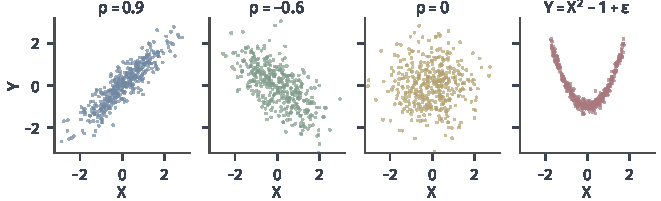
\includegraphics[width=112mm]{figures/01-basic-mathematics/05-probability-and-statistics-basics/matplotlib/rvec-correlation/figure.pdf}
  \caption{不同相关系数下的散点，每幅$400$个模拟点（固定随机种子）。前三幅中$X$与$Y$都是标准高斯变量，相关系数分别为$0.9$、$-0.6$和$0$。第四幅中$X$在$[-\sqrt3,\sqrt3]$上均匀分布，$Y=X^2-1$再加小噪声，相关系数为零，但$Y$几乎由$X$决定。}
  \label{fig:rvec-correlation}
\end{figure}

\begin{example}[两个例子的相关系数]
\label{ex:rvec-correlation-values}
示例~\ref{ex:rvec-study-table}中$\operatorname{Var}(X)=\mathbb EX^2-1=(0.4+4\times0.3)-1=0.6$，$\operatorname{Var}(Y)=0.6\times0.4=0.24$，故
$\rho=0.15/\sqrt{0.6\times0.24}\approx0.40$。

示例~\ref{ex:rvec-square-density}中，$\mathbb E[XY]=\int_0^1\!\int_0^1xy(x+y)\,\mathrm dy\,\mathrm dx=1/3$，$\mathbb EX^2=\int_0^1x^2(x+1/2)\,\mathrm dx=5/12$。于是
\[
 \operatorname{Cov}(X,Y)=\frac13-\Bigl(\frac7{12}\Bigr)^2=-\frac1{144},\qquad
 \operatorname{Var}(X)=\frac5{12}-\frac{49}{144}=\frac{11}{144},
\]
相关系数为$-1/11\approx-0.09$。密度$x+y$在两个分量都大时较大，看起来像“同向”，但在这个密度下，一个分量偏大时，另一个分量的条件分布会向下移动（第~\ref{sec:rvec-conditioning}节会算出这一点），总体上呈现微弱的负相关。直观印象需要通过计算核对。
\end{example}

\subsection{协方差矩阵}
\label{sec:rvec-covariance-matrix}

\paragraph{定义与半正定性}
$d$个分量两两之间都有协方差，把它们排成矩阵便于统一计算。设各分量二阶矩有限，定义\term{协方差矩阵}（covariance matrix）
\[
 \bm\Sigma=\operatorname{Cov}(\bm X)=\mathbb E\bigl[(\bm X-\bm\mu)(\bm X-\bm\mu)^{\top}\bigr],
 \qquad \bm\Sigma_{i,j}=\operatorname{Cov}(X_i,X_j),
\]
其中矩阵的期望逐元素计算。对角元是各分量的方差，非对角元是协方差。

\begin{theorem}[协方差矩阵的性质]
\label{thm:rvec-covariance-psd}
协方差矩阵对称半正定。对任意常向量$\bm a,\bm b\in\mathbb R^d$，
\[
 \operatorname{Var}(\bm a^{\top}\bm X)=\bm a^{\top}\bm\Sigma\bm a\ge0,\qquad
 \operatorname{Cov}(\bm a^{\top}\bm X,\bm b^{\top}\bm X)=\bm a^{\top}\bm\Sigma\bm b .
\]
\end{theorem}

\begin{proof}
对称性来自$\operatorname{Cov}(X_i,X_j)=\operatorname{Cov}(X_j,X_i)$。由均值向量的线性性，$\bm a^{\top}\bm X-\mathbb E(\bm a^{\top}\bm X)=\bm a^{\top}(\bm X-\bm\mu)$，同理处理$\bm b$。两个标量相乘可写成
\[
 \bm a^{\top}(\bm X-\bm\mu)\,(\bm X-\bm\mu)^{\top}\bm b ,
\]
它是矩阵$(\bm X-\bm\mu)(\bm X-\bm\mu)^{\top}$各元素的线性组合，取期望后得到$\bm a^{\top}\bm\Sigma\bm b$。取$\bm b=\bm a$得方差公式；方差非负，所以$\bm\Sigma$半正定。
\end{proof}

这个定理把任意线性组合的方差交给一个矩阵计算，式~\eqref{eq:rvec-variance-of-combination}是$d=2$的特例。示例~\ref{ex:rvec-study-table}中
\[
 \bm\Sigma=\begin{bmatrix}0.6&0.15\\0.15&0.24\end{bmatrix}.
\]
例如取$\bm a=(1,-2)^{\top}$，得$\operatorname{Var}(X-2Y)=\bm a^{\top}\bm\Sigma\bm a=0.6-4\times0.15+4\times0.24=0.96$。

\paragraph{多项计数的负协方差}
多项分布的计数之和固定，这个约束会体现在协方差上。由边缘分布$N_k\sim\operatorname{Bin}(n,\pi_k)$，$\operatorname{Var}(N_k)=n\pi_k(1-\pi_k)$。对$j\neq k$，把类别$j$与$k$合并成一类，$N_j+N_k$就是$n$次试验中落入合并类别的次数，服从$\operatorname{Bin}(n,\pi_j+\pi_k)$。由式~\eqref{eq:rvec-variance-of-combination}，
\[
 n(\pi_j+\pi_k)(1-\pi_j-\pi_k)=n\pi_j(1-\pi_j)+n\pi_k(1-\pi_k)+2\operatorname{Cov}(N_j,N_k).
\]
展开左边并消去相同项，得到
\[
 \operatorname{Cov}(N_j,N_k)=-n\pi_j\pi_k ,\qquad
 \bm\Sigma=n\bigl(\operatorname{diag}(\bm\pi)-\bm\pi\bm\pi^{\top}\bigr).
\]
协方差为负的原因很直接：总次数固定，某一类多出现一次，其余类别可分配的次数就少一次。示例~\ref{ex:rvec-multinomial}的参数给出
\[
 \bm\Sigma=\begin{bmatrix}1&-0.6&-0.4\\-0.6&0.84&-0.24\\-0.4&-0.24&0.64\end{bmatrix},
\]
每行之和都是零。

\paragraph{退化与线性关系}
行和为零说明$\bm\Sigma\bm 1=\bm0$，其中$\bm1$是全一向量。按定理~\ref{thm:rvec-covariance-psd}，$\operatorname{Var}(\bm1^{\top}\bm N)=\bm1^{\top}\bm\Sigma\bm1=0$，这正是$N_1+\cdots+N_K=n$恒成立。一般地，若$\bm a\neq\bm0$使$\bm a^{\top}\bm\Sigma\bm a=0$，则$\bm a^{\top}\bm X$方差为零，由定理~\ref{thm:rvec-correlation-bound}证明中的论证，它以概率$1$等于常数$\bm a^{\top}\bm\mu$。因此，协方差矩阵奇异，恰好对应分量之间以概率$1$成立的线性关系；这时$\bm X$的取值集中在一个超平面上。超平面在$\mathbb R^d$中的体积为零，任何联合密度在其上的积分都为零，所以这样的$\bm X$不可能有$d$维联合密度。

\section{随机变量的独立性}
\label{sec:rvec-independence}

联合分布中最简单的一种结构，是知道一个变量的取值完全不改变另一个变量的概率。第~\ref{sec:prob-event-independence}节已经对事件定义了独立性；本节把它推广到随机变量，并比较它与不相关的区别。

\subsection{独立性的定义与判定}

\paragraph{定义}
随机变量的独立应当意味着：关于$X$的任何事件与关于$Y$的任何事件都相互独立。

\begin{definition}[随机变量的独立性]
称随机变量$X$与$Y$\term{独立}（independent），记为$X\perp Y$，如果对所有能够计算概率的实数集合$A,B$（例如区间及其有限并），
\[
 \mathbb P(X\in A,\,Y\in B)=\mathbb P(X\in A)\,\mathbb P(Y\in B).
\]
\end{definition}

把$X,Y$换成随机向量、$A,B$换成相应维数空间中的集合，就得到两个随机向量独立的定义，下面的判定也照样成立。当$\mathbb P(X\in A)>0$时，等式等价于$\mathbb P(Y\in B\mid X\in A)=\mathbb P(Y\in B)$：无论得知$X$落在哪个范围，$Y$的概率都不变。这个定义对每一对集合都要检查，实际判定时通常改用质量函数或密度。

\begin{theorem}[独立性的判定]
\label{thm:rvec-independence-criteria}
\begin{enumerate}
 \item 若$X,Y$是离散随机变量，则$X\perp Y$当且仅当对所有$x,y$，$p_{X,Y}(x,y)=p_X(x)p_Y(y)$。
 \item 若$(X,Y)$具有联合密度，则$X\perp Y$当且仅当$f_X(x)f_Y(y)$也是$(X,Y)$的联合密度，即可以取$f_{X,Y}(x,y)=f_X(x)f_Y(y)$。
\end{enumerate}
\end{theorem}

\begin{proof}
离散情形。必要性取$A=\{x\}$，$B=\{y\}$即可。充分性：
\[
 \mathbb P(X\in A,Y\in B)=\sum_{x\in A}\sum_{y\in B}p_X(x)p_Y(y)
 =\Bigl(\sum_{x\in A}p_X(x)\Bigr)\Bigl(\sum_{y\in B}p_Y(y)\Bigr).
\]
密度情形。若$f_{X,Y}=f_Xf_Y$，对区间$A,B$按累次积分，
\[
 \iint_{A\times B}f_X(x)f_Y(y)\,\mathrm dx\,\mathrm dy=\int_Af_X(x)\,\mathrm dx\int_Bf_Y(y)\,\mathrm dy ,
\]
这正是独立性的等式；有限并的情形逐块相加。反过来，若$X\perp Y$，则对任意矩形，
\[
 \mathbb P(a_1<X\le b_1,\,a_2<Y\le b_2)=\int_{a_1}^{b_1}f_X(x)\,\mathrm dx\int_{a_2}^{b_2}f_Y(y)\,\mathrm dy ,
\]
即函数$f_Xf_Y$给出与$(X,Y)$相同的矩形概率，因而可以作为联合密度。
\end{proof}

密度只在不影响任何积分的个别点或曲线上可以任意改动，所以第二条说的是“可以取成乘积”，而不是要求在每一点都相等。

\paragraph{按乘积形式判别}
实际判别时，常检查联合密度能否在整个平面上写成两个非负函数之积$g(x)h(y)$。若能，那么分别对$y$和$x$积分可知$f_X$与$g$、$f_Y$与$h$只差常数因子，两个常数之积为$1$，因而$X\perp Y$。例如在$x,y>0$上$f_{X,Y}(x,y)=6e^{-2x-3y}$，它可写成$2e^{-2x}$与$3e^{-3y}$之积，所以$X\sim\operatorname{Exp}(2)$与$Y\sim\operatorname{Exp}(3)$独立。

乘积分解必须连同取值范围一起检查。设$(X,Y)$在三角形$\{0<y<x<1\}$上均匀分布，密度在三角形内恒为$2$，看起来不含$x$与$y$的交叉项。但边缘密度为$f_X(x)=2x$，$f_Y(y)=2(1-y)$；在点$(1/4,3/4)$处联合密度为零，乘积却是$1/2\times1/2=1/4$。整块取值范围不是乘积形状时，指示函数$\mathbb{I}\{y<x\}$本身就是不能分开的交叉项。离散情形同理：图~\ref{fig:rvec-joint-table}中$p_{X,Y}(0,0)=0.20$，而$p_X(0)p_Y(0)=0.3\times0.4=0.12$，所以复习次数与考试结果不独立。

\paragraph{函数变换与乘积的期望}
独立性经过各自的函数变换后仍然保持。设$X\perp Y$，$g,h$为实函数。记$g^{-1}(A)=\{x:g(x)\in A\}$，则
\[
\begin{aligned}
 \mathbb P\bigl(g(X)\in A,\,h(Y)\in B\bigr)&=\mathbb P\bigl(X\in g^{-1}(A),\,Y\in h^{-1}(B)\bigr)\\
 &=\mathbb P\bigl(g(X)\in A\bigr)\,\mathbb P\bigl(h(Y)\in B\bigr),
\end{aligned}
\]
只要这些原像集合仍在我们能计算概率的范围内。例如$X^2$与$e^{Y}$独立。

\begin{theorem}[独立变量乘积的期望]
\label{thm:rvec-product-expectation}
设$X\perp Y$，$\mathbb E|g(X)|<\infty$，$\mathbb E|h(Y)|<\infty$。则$g(X)h(Y)$的期望有限，且
\[
 \mathbb E\bigl[g(X)h(Y)\bigr]=\mathbb E\,g(X)\;\mathbb E\,h(Y).
\]
\end{theorem}

\begin{proof}
离散情形，由独立性的判定，
\[
\begin{aligned}
 \mathbb E\bigl[g(X)h(Y)\bigr]&=\sum_x\sum_yg(x)h(y)p_X(x)p_Y(y)\\
 &=\Bigl(\sum_xg(x)p_X(x)\Bigr)\Bigl(\sum_yh(y)p_Y(y)\Bigr).
\end{aligned}
\]
先对绝对值做同样的计算，得到$\mathbb E|g(X)h(Y)|=\mathbb E|g(X)|\,\mathbb E|h(Y)|<\infty$；二重级数绝对收敛，才允许上面重新排列求和次序。密度情形把求和换成累次积分，论证相同。
\end{proof}

只知道乘积$g(X)h(Y)$的期望有限是不够的：若$g\equiv0$，乘积期望为零，而$\mathbb E\,h(Y)$可能根本不存在，右边就没有意义。对上面的指数例子，$\mathbb E[XY^2]=\mathbb EX\cdot\mathbb EY^2=\frac12\times\frac2{9}=\frac19$，其中用到$Y\sim\operatorname{Exp}(3)$时$\mathbb EY^2=2/3^2$。

\subsection{两两独立与相互独立}

\paragraph{多个变量的独立}
多个变量时，有两种自然但强弱不同的要求。

\begin{definition}[相互独立与两两独立]
称随机变量$X_1,\ldots,X_n$\term{相互独立}（mutually independent），如果对所有能够计算概率的实数集合$A_1,\ldots,A_n$，
\[
 \mathbb P(X_1\in A_1,\ldots,X_n\in A_n)=\prod_{i=1}^n\mathbb P(X_i\in A_i).
\]
若只要求其中每一对变量独立，称它们\term{两两独立}（pairwise independent）。
\end{definition}

在相互独立的等式中取部分$A_i=\mathbb R$，相应因子变成$1$，就得到任意一部分变量的乘积关系。这与第~\ref{sec:prob-event-independence}节对事件“所有子组都满足乘法关系”的要求一致，所以相互独立蕴含两两独立。离散或密度模型中，相互独立等价于联合质量函数或联合密度可以取成$n$个边缘的乘积，证明与定理~\ref{thm:rvec-independence-criteria}相同。今后说“独立同分布”的变量，指的总是相互独立。

相互独立还有一个常用推论：把变量分成互不相交的几组，各组的函数仍相互独立。以离散情形为例，若$X_1,X_2,X_3$相互独立，则
\[
\begin{aligned}
 \mathbb P\bigl(X_1+X_2=s,\,X_3=v\bigr)&=\sum_{x_1+x_2=s}p_{X_1}(x_1)p_{X_2}(x_2)p_{X_3}(v)\\
 &=\mathbb P(X_1+X_2=s)\,\mathbb P(X_3=v),
\end{aligned}
\]
所以$X_1+X_2\perp X_3$。第~\ref{sec:rvec-transforms}节按这种方式逐个累加独立变量。

\paragraph{异或反例}
两两独立却不能保证相互独立。令$X,Y$独立，都等可能取$0$或$1$，再令$Z=X\oplus Y$为两者的\term{异或}（exclusive OR）：$X,Y$相同时$Z=0$，不同时$Z=1$。四种等可能结果列在表~\ref{tab:rvec-xor}中。

\begin{table}[htbp]
  \centering
  \caption{异或构造的四种等可能结果。任意两列取遍四种组合各一次，第三列却由前两列唯一确定。}
  \label{tab:rvec-xor}
  \begin{tabular}{cccc}
    \toprule
    $X$ & $Y$ & $Z=X\oplus Y$ & 概率\\
    \midrule
    $0$ & $0$ & $0$ & $1/4$\\
    $0$ & $1$ & $1$ & $1/4$\\
    $1$ & $0$ & $1$ & $1/4$\\
    $1$ & $1$ & $0$ & $1/4$\\
    \bottomrule
  \end{tabular}
\end{table}

逐对检查。$Z$取$0$与$1$各有两行，故$\mathbb P(Z=1)=1/2$。$(X,Y)$独立是假设。对$(X,Z)$，表中$(X,Z)$的四种组合$(0,0),(0,1),(1,1),(1,0)$各出现一次，所以$\mathbb P(X=x,Z=z)=1/4=\mathbb P(X=x)\mathbb P(Z=z)$；$(Y,Z)$同理。三个变量因此两两独立。但
\[
 \mathbb P(X=1,Y=1,Z=1)=0\neq\frac18=\mathbb P(X=1)\mathbb P(Y=1)\mathbb P(Z=1),
\]
三者不相互独立。单看$X$或单看$Y$，都得不到关于$Z$的任何信息；两者合在一起却完全决定$Z$。分类问题中，两个特征各自与类别无关、合起来却决定类别，正是这种结构。

\subsection{独立与不相关}

\paragraph{独立推出不相关}
协方差为零的两个变量称为\term{不相关}（uncorrelated）。独立性比它强。

\begin{theorem}[独立变量不相关]
\label{thm:rvec-independent-uncorrelated}
若$X\perp Y$且二者二阶矩有限，则$\operatorname{Cov}(X,Y)=0$。
\end{theorem}

\begin{proof}
二阶矩有限蕴含$\mathbb E|X-\mu_X|<\infty$与$\mathbb E|Y-\mu_Y|<\infty$。对$g(x)=x-\mu_X$、$h(y)=y-\mu_Y$用定理~\ref{thm:rvec-product-expectation}，
$\operatorname{Cov}(X,Y)=\mathbb E[X-\mu_X]\,\mathbb E[Y-\mu_Y]=0\cdot0=0$。
\end{proof}

在定理~\ref{thm:rvec-covariance-psd}中取$\bm a$为全一向量，$\operatorname{Var}(X_1+\cdots+X_n)$等于全部方差与全部协方差之和；因此两两不相关的变量满足$\operatorname{Var}(X_1+\cdots+X_n)=\operatorname{Var}(X_1)+\cdots+\operatorname{Var}(X_n)$。这里只需要每一对协方差为零，两两独立已经足够。例如$n$个独立$\operatorname{Bernoulli}(p)$变量之和的方差为$np(1-p)$，与第~\ref{sec:prob-discrete-models}节二项分布的方差一致。

\paragraph{不相关不推出独立}
反方向一般不成立。令$X$在$\{-1,0,1\}$上等可能取值，$Y=X^2$。由对称性$\mathbb EX=\mathbb EX^3=0$，所以
\[
 \operatorname{Cov}(X,Y)=\mathbb E[X^3]-\mathbb EX\,\mathbb EX^2=0 .
\]
但$\mathbb P(X=0,Y=0)=1/3$，而$\mathbb P(X=0)\mathbb P(Y=0)=1/3\times1/3=1/9$，二者不独立；实际上$Y$由$X$完全决定。同样的论证适用于任何关于零对称、三阶矩有限的$X$。图~\ref{fig:rvec-correlation}第四幅就是连续版本：抽到的$X$越远离零，$Y$越大，这种依赖对正负两侧是对称的，没有“$X$增大时$Y$随之增大或减小”的线性趋势，协方差把它完全漏掉了。

因此，协方差为零只排除了线性关联。只有在额外的模型假设下，例如第~\ref{sec:rvec-gaussian}节的联合高斯条件，不相关才能推出独立。

\section{条件概率与条件分布}
\label{sec:rvec-conditioning}
\label{sec:rv-conditional-distribution}

独立表示一个变量不提供关于另一个变量的信息。多数情况下并非如此：得知学生复习了两次，他通过考试的概率就应当提高。本节先在事件层面建立汇总与反推的两个公式，再把条件概率推广为条件分布，并研究条件分布的均值、方差以及条件独立。

\subsection{全概率公式与Bayes公式}
\label{sec:rvec-bayes-formula}

\paragraph{全概率公式}
回顾第~\ref{sec:prob-conditional-probability}节：$\mathbb P(B)>0$时，$\mathbb P(A\mid B)=\mathbb P(A\cap B)/\mathbb P(B)$，由此得到乘法公式$\mathbb P(A\cap B)=\mathbb P(A\mid B)\mathbb P(B)$。设某工厂的产品来自三条产线，各产线的产量占比和次品率都已知，我们想知道任取一件产品是次品的概率。这类问题的共同结构是：总体被分成若干互斥的情形，每种情形下的条件概率已知，需要把它们汇总起来。

\begin{theorem}[全概率公式]
\label{thm:rvec-total-probability}
设事件$B_1,\ldots,B_m$两两互斥，并集为整个样本空间，且每个$\mathbb P(B_i)>0$。则对任意事件$A$，
\[
 \mathbb P(A)=\sum_{i=1}^m\mathbb P(A\mid B_i)\,\mathbb P(B_i).
\]
\end{theorem}

\begin{proof}
$B_1,\ldots,B_m$覆盖全部结果且互不相交，所以$A=\bigcup_i(A\cap B_i)$，各部分互斥。由可加性$\mathbb P(A)=\sum_i\mathbb P(A\cap B_i)$，再对每一项用乘法公式即得。
\end{proof}

这个公式称为\term{全概率公式}（law of total probability）。可数多个情形时，可数可加性给出同样的结论。它把一个不易直接计算的概率，拆成“先确定处于哪种情形，再在该情形下计算”的加权平均。

\begin{example}[三条产线的次品率]
\label{ex:rvec-production-lines}
设产品来自三条产线，记事件$B_k$为“产品来自第$k$条产线”，$D$为“产品是次品”。产量占比为$\mathbb P(B_1)=0.5$、$\mathbb P(B_2)=0.3$、$\mathbb P(B_3)=0.2$，次品率为$\mathbb P(D\mid B_1)=0.01$、$\mathbb P(D\mid B_2)=0.02$、$\mathbb P(D\mid B_3)=0.04$（教学数据）。由全概率公式，
\[
 \mathbb P(D)=0.5\times0.01+0.3\times0.02+0.2\times0.04=0.005+0.006+0.008=0.019 .
\]
图~\ref{fig:rvec-bayes-tree}把这个计算画成树：每条路径上的概率相乘，得到“来自某产线且是次品”的概率，再把三条次品路径相加。
\end{example}

\begin{figure*}[htbp]
  \centering
  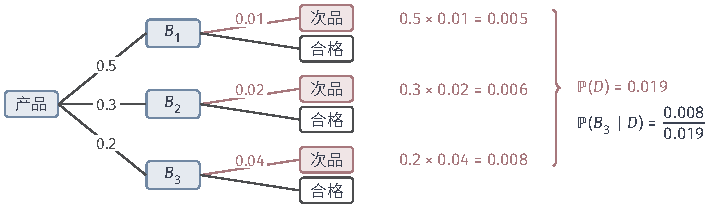
\includegraphics[width=121.6mm]{figures/01-basic-mathematics/05-probability-and-statistics-basics/tikz/rvec-bayes-tree/figure.pdf}
  \caption{全概率公式与Bayes公式的树状图。第一层分支是产品来自三条产线的概率，第二层是各产线的次品率。沿路径相乘得到三个联合概率$\mathbb P(B_k\cap D)$，相加得到$\mathbb P(D)=0.019$；其中第三条路径所占的比例就是$\mathbb P(B_3\mid D)$。}
  \label{fig:rvec-bayes-tree}
\end{figure*}

\paragraph{Bayes公式}
全概率公式由原因推出结果。实际中常常需要反过来问：已经发现一件次品，它来自第三条产线的概率是多少？已知的是$\mathbb P(D\mid B_k)$，要求的是方向相反的$\mathbb P(B_k\mid D)$。

\begin{theorem}[Bayes公式]
\label{thm:rvec-bayes}
在定理~\ref{thm:rvec-total-probability}的条件下，若$\mathbb P(A)>0$，则对每个$j$，
\[
 \mathbb P(B_j\mid A)=\frac{\mathbb P(A\mid B_j)\,\mathbb P(B_j)}{\sum_{i=1}^m\mathbb P(A\mid B_i)\,\mathbb P(B_i)} .
\]
\end{theorem}

\begin{proof}
由条件概率的定义与乘法公式，
\[
 \mathbb P(B_j\mid A)=\frac{\mathbb P(A\cap B_j)}{\mathbb P(A)}=\frac{\mathbb P(A\mid B_j)\,\mathbb P(B_j)}{\mathbb P(A)} ,
\]
再用全概率公式展开分母。
\end{proof}

这个公式称为\term{Bayes公式}（Bayes' formula）。$\mathbb P(B_j)$是观测之前对各情形的概率，称为\term{先验概率}（prior probability）；$\mathbb P(B_j\mid A)$是得知$A$发生后重新计算的概率，称为\term{后验概率}（posterior probability）。公式说明：后验概率正比于“先验概率乘以该情形下观测到$A$的概率”，分母只负责归一化，使全部后验概率之和为$1$。

\begin{example}[次品来自哪条产线]
\label{ex:rvec-production-bayes}
续示例~\ref{ex:rvec-production-lines}。三条次品路径的概率是$0.005$、$0.006$、$0.008$，除以总和$0.019$，
\[
 \mathbb P(B_1\mid D)\approx0.263,\qquad \mathbb P(B_2\mid D)\approx0.316,\qquad \mathbb P(B_3\mid D)\approx0.421 .
\]
第三条产线只生产两成产品，却贡献了四成以上的次品，因为它的次品率最高。分母必须汇总全部情形：若计算时漏掉第二条产线，会误得$\mathbb P(B_3\mid D)=0.008/0.013\approx0.615$。被漏掉的情形同样可能产生次品，它的贡献不计入分母，其余情形的后验概率就被系统地高估。
\end{example}

先验概率的影响有时与直觉相差很大。设某种疾病的患病率为$1\%$，检测对患者呈阳性的概率为$0.9$，对未患病者误报阳性的概率为$0.05$。阳性的概率为$0.01\times0.9+0.99\times0.05=0.0585$，于是阳性者确实患病的概率只有$0.009/0.0585\approx0.154$。检测本身相当灵敏，但未患病的人数是患者的$99$倍，他们中少量的误报在阳性结果里仍占多数。

\subsection{条件分布}

\paragraph{离散情形：按行归一化}
把条件概率用于随机变量的取值事件，就得到条件分布。对离散变量，只要$p_X(x)>0$，事件$\{X=x\}$有正概率，可以直接定义
\[
 p_{Y\mid X}(y\mid x)=\mathbb P(Y=y\mid X=x)=\frac{p_{X,Y}(x,y)}{p_X(x)} .
\]
固定$x$，它对$y$非负且和为$1$，是一个质量函数，称为给定$X=x$时$Y$的\term{条件分布}（conditional distribution），$p_{Y\mid X}$称为\term{条件质量函数}（conditional probability mass function）。在二维概率表中，这就是取出$X=x$那一行，再除以该行之和，如图~\ref{fig:rvec-joint-table}(b)所示。

对示例~\ref{ex:rvec-study-table}，三行归一化后，给定$X=0,1,2$时$Y=1$的条件概率依次为
\[
 \frac{0.10}{0.30}=\frac13,\qquad \frac{0.25}{0.40}=0.625,\qquad \frac{0.25}{0.30}=\frac56 .
\]
无条件时$\mathbb P(Y=1)=0.6$；得知复习次数以后，这个概率在$1/3$到$5/6$之间变化。这正是$X$与$Y$不独立的表现：若二者独立，每一行归一化后都等于$p_Y$。

\paragraph{连续情形：条件密度}
具有联合密度时，单点事件$\{X=x\}$的概率为零，上面的除法不能照搬到事件上。我们改为在密度层面作同样的“取一条、再归一化”：对$f_X(x)>0$的$x$，定义\term{条件密度}（conditional density）
\[
 f_{Y\mid X}(y\mid x)=\frac{f_{X,Y}(x,y)}{f_X(x)} .
\]
固定$x$，它对$y$非负，积分为$f_X(x)/f_X(x)=1$，是一个密度；给定$X=x$时$Y$落在$B$中的条件概率规定为$\int_Bf_{Y\mid X}(y\mid x)\,\mathrm dy$。对示例~\ref{ex:rvec-square-density}，
\[
 f_{Y\mid X}(y\mid x)=\frac{x+y}{x+1/2},\qquad 0\le y\le1 .
\]
$x=0$时为$2y$，质量集中在$y$较大处；$x=1$时为$\frac23(1+y)$，明显平坦得多。

\paragraph{乘积关系与密度的Bayes公式}
两种情形都可以把定义改写为乘积：
\[
\begin{aligned}
 p_{X,Y}(x,y)&=p_X(x)\,p_{Y\mid X}(y\mid x)=p_Y(y)\,p_{X\mid Y}(x\mid y),\\
 f_{X,Y}(x,y)&=f_X(x)\,f_{Y\mid X}(y\mid x)=f_Y(y)\,f_{X\mid Y}(x\mid y).
\end{aligned}
\]
联合分布等于“边缘分布乘以条件分布”，这是第~\ref{sec:rvec-generation}节条件生成的依据。两种分解联立，再用边缘化展开分母，得到随机变量形式的Bayes公式，例如密度情形
\[
 f_{X\mid Y}(x\mid y)=\frac{f_{Y\mid X}(y\mid x)\,f_X(x)}{\int f_{Y\mid X}(y\mid t)\,f_X(t)\,\mathrm dt} ,
\]
离散情形把积分换成求和。与事件形式一样，分子给出各个$x$的相对权重，分母负责归一化。

\paragraph{条件密度的含义}
条件密度不是两个零概率事件之比，它可以理解为“在$x$附近一条窄带中取条件”的极限。设$f_{X,Y}$连续，$f_X(x)>0$。对$h>0$，
\[
 \mathbb P(Y\le y\mid x\le X\le x+h)
 =\frac{\frac1h\int_x^{x+h}\bigl(\int_{-\infty}^yf_{X,Y}(s,t)\,\mathrm dt\bigr)\mathrm ds}{\frac1h\int_x^{x+h}f_X(s)\,\mathrm ds} .
\]
分子分母都是正概率事件的概率除以$h$。令$h\to0$，由微积分基本定理，分子趋于$\int_{-\infty}^yf_{X,Y}(x,t)\,\mathrm dt$，分母趋于$f_X(x)$，比值正是$\int_{-\infty}^yf_{Y\mid X}(t\mid x)\,\mathrm dt$。这个极限依赖于“用竖直窄带逼近直线$X=x$”的方式；若改用其他形状的邻域逼近同一条零概率曲线，可能得到不同的结果。在本部分的模型中，我们始终按上面的密度比计算，一般情形的严格处理留到卷二。

\subsection{条件期望}
\label{sec:rvec-conditional-expectation}

\paragraph{条件均值与条件期望}
条件分布本身仍是一个分布，可以计算它的均值。给定$X=x$，若相应求和或积分绝对收敛，定义
\[
 \mathbb E[Y\mid X=x]=\sum_yy\,p_{Y\mid X}(y\mid x)
 \quad\text{或}\quad
 \mathbb E[Y\mid X=x]=\int y\,f_{Y\mid X}(y\mid x)\,\mathrm dy ,
\]
称为给定$X=x$时$Y$的\term{条件期望}（conditional expectation）。它随$x$变化，记为$m(x)=\mathbb E[Y\mid X=x]$，是一个普通函数。

需要区分两个对象。对每个固定的$x$，$m(x)$是一个数；把随机变量$X$代入，得到随机变量$m(X)$，记为$\mathbb E[Y\mid X]$。后者在试验结果揭晓、$X$取值为$x$时取值$m(x)$，它是$X$的函数，因而不再含有$X$以外的随机性。类似地，$\mathbb E[g(Y)\mid X=x]$按条件分布计算$g(Y)$的均值；已知的因子可以提出，$\mathbb E[h(X)Y\mid X=x]=h(x)m(x)$，因为在给定$X=x$的条件分布中$h(X)$就是常数$h(x)$。

\begin{example}[两个例子的条件期望]
\label{ex:rvec-conditional-means}
示例~\ref{ex:rvec-study-table}中$Y$只取$0,1$，条件均值等于$Y=1$的条件概率：$m(0)=1/3$，$m(1)=5/8$，$m(2)=5/6$。于是$\mathbb E[Y\mid X]$是一个以概率$0.3,0.4,0.3$分别取$1/3,5/8,5/6$的随机变量。

示例~\ref{ex:rvec-square-density}中，
\[
 m(x)=\int_0^1y\,\frac{x+y}{x+1/2}\,\mathrm dy=\frac{x/2+1/3}{x+1/2}=\frac{3x+2}{6x+3},
\]
从$m(0)=2/3$单调减到$m(1)=5/9$。$X$越大，$Y$的条件均值越小，这解释了示例~\ref{ex:rvec-correlation-values}中的负相关。
\end{example}

\paragraph{全期望公式}
各组条件均值按组的概率加权平均，应当回到总体均值。

\begin{theorem}[全期望公式]
\label{thm:rvec-total-expectation}
若$\mathbb E|Y|<\infty$，则$\mathbb E\bigl[\mathbb E[Y\mid X]\bigr]=\mathbb EY$。
\end{theorem}

\begin{proof}
离散情形，用乘积关系$p_X(x)p_{Y\mid X}(y\mid x)=p_{X,Y}(x,y)$，
\[
 \mathbb E\,m(X)=\sum_xp_X(x)\sum_yy\,p_{Y\mid X}(y\mid x)=\sum_x\sum_yy\,p_{X,Y}(x,y)=\mathbb EY .
\]
$\mathbb E|Y|<\infty$保证二重级数绝对收敛，求和次序可以交换。密度情形把求和换成累次积分，同样有
\[
 \int f_X(x)\int y\,f_{Y\mid X}(y\mid x)\,\mathrm dy\,\mathrm dx=\iint y\,f_{X,Y}(x,y)\,\mathrm dy\,\mathrm dx=\mathbb EY .
\]
\end{proof}

这就是\term{全期望公式}（law of total expectation），它是全概率公式在均值上的对应：先在每一组内求平均，再按组的概率加权平均。示例~\ref{ex:rvec-conditional-means}中，$0.3\times\frac13+0.4\times\frac58+0.3\times\frac56=0.1+0.25+0.25=0.6=\mathbb EY$；连续例子中$m(x)f_X(x)=x/2+1/3$，积分得$1/4+1/3=7/12$，也等于$\mathbb EY$。

\subsection{条件方差}
\label{sec:rvec-conditional-variance}

\paragraph{定义与含义}
条件均值描述得知$X$以后$Y$的中心，还需要描述围绕这个中心的剩余波动。设$\mathbb EY^2<\infty$，定义\term{条件方差}（conditional variance）
\[
 \operatorname{Var}(Y\mid X=x)=\mathbb E\bigl[(Y-m(x))^2\bigm| X=x\bigr]=\mathbb E[Y^2\mid X=x]-m(x)^2 ,
\]
第二个等号是一元方差计算公式在条件分布上的应用。把$X$代入得到随机变量$\operatorname{Var}(Y\mid X)$。它描述知道$X$以后仍无法消除的不确定性。示例~\ref{ex:rvec-study-table}中，给定$X=x$时$Y$服从$\operatorname{Bernoulli}(m(x))$，所以
\[
\begin{gathered}
 \operatorname{Var}(Y\mid X=0)=\frac13\cdot\frac23=\frac29,\qquad
 \operatorname{Var}(Y\mid X=1)=\frac58\cdot\frac38=\frac{15}{64},\\
 \operatorname{Var}(Y\mid X=2)=\frac56\cdot\frac16=\frac5{36}.
\end{gathered}
\]
三者分别约为$0.222$、$0.234$、$0.139$，都小于$\operatorname{Var}(Y)=0.24$，而且随$x$变化。

\paragraph{全方差公式}
总波动与“组内波动”“组间波动”之间有一个精确的分解。

\begin{theorem}[全方差公式]
\label{thm:rvec-total-variance}
若$\mathbb EY^2<\infty$，则
\[
 \operatorname{Var}(Y)=\mathbb E\bigl[\operatorname{Var}(Y\mid X)\bigr]+\operatorname{Var}\bigl(\mathbb E[Y\mid X]\bigr).
\]
\end{theorem}

\begin{proof}
记$\mu=\mathbb EY$。把偏离拆成两段：$Y-\mu=\bigl(Y-m(X)\bigr)+\bigl(m(X)-\mu\bigr)$。平方后取期望，交叉项为
\[
\begin{aligned}
 &\mathbb E\bigl[(Y-m(X))(m(X)-\mu)\bigr]\\
 &\quad=\sum_xp_X(x)\bigl(m(x)-\mu\bigr)\sum_y\bigl(y-m(x)\bigr)p_{Y\mid X}(y\mid x)=0 ,
\end{aligned}
\]
因为内层和等于$m(x)-m(x)=0$。第一段平方的期望为
\[
 \sum_xp_X(x)\operatorname{Var}(Y\mid X=x)=\mathbb E\bigl[\operatorname{Var}(Y\mid X)\bigr];
\]
由全期望公式$\mathbb E\,m(X)=\mu$，第二段平方的期望就是$\operatorname{Var}(m(X))$。密度情形把求和换成积分。
\end{proof}

这就是\term{全方差公式}（law of total variance）。第一项是各组内部波动的平均，第二项是各组均值彼此不同造成的波动。图~\ref{fig:rvec-total-variance}中$X$等可能取$1,2,3$，给定$X=k$时$Y\sim\mathcal N(2k-1,1)$。每组内部的方差都是$1$，三组均值$1,3,5$围绕总均值$3$的方差是$(4+0+4)/3=8/3$，所以$\operatorname{Var}(Y)=1+8/3=11/3$。只看任一组都会低估总体的分散程度。

\begin{figure}[htbp]
  \centering
  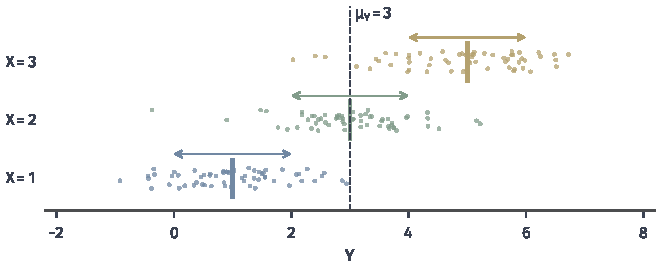
\includegraphics[width=112mm]{figures/01-basic-mathematics/05-probability-and-statistics-basics/matplotlib/rvec-total-variance/figure.pdf}
  \caption{全方差公式的组内与组间两部分。$X$等可能取$1,2,3$，给定$X=k$时$Y\sim\mathcal N(2k-1,1)$；每组画出$60$个模拟值（固定随机种子，纵向抖动只为避免重叠）。粗竖线是组均值，双箭头标出组均值左右各一个条件标准差，虚线是总均值$3$。组内方差为$1$，组间方差为$8/3$，总方差为$11/3$。}
  \label{fig:rvec-total-variance}
\end{figure}

对示例~\ref{ex:rvec-study-table}，组内部分为$0.3\times\frac29+0.4\times\frac{15}{64}+0.3\times\frac5{36}\approx0.2021$；组间部分为$0.3\times\frac19+0.4\times\frac{25}{64}+0.3\times\frac{25}{36}-0.6^2\approx0.0379$，两者之和恰为$0.24$。复习次数解释的只是考试结果总波动中约$16\%$的部分。两项都非负，所以$\mathbb E[\operatorname{Var}(Y\mid X)]\le\operatorname{Var}(Y)$：平均而言，获得信息不会增加波动。但在个别取值$x$上，条件方差可以大于无条件方差：若某门考试总体通过率为$0.9$，而其中一组学生的通过率只有$0.5$，这一组的条件方差$0.25$就大于总体方差$0.09$。

\subsection{条件独立}

\paragraph{定义}
条件分布也可以有独立结构。先固定第三个变量，再问两个变量是否独立，就得到条件独立。

\begin{definition}[条件独立]
设$(X,Y,Z)$是离散随机向量。若对所有满足$p_Z(z)>0$的$z$以及所有$x,y$，
\[
 p_{X,Y\mid Z}(x,y\mid z)=p_{X\mid Z}(x\mid z)\,p_{Y\mid Z}(y\mid z),
\]
则称在给定$Z$的条件下$X$与$Y$\term{条件独立}（conditionally independent），记为$X\perp Y\mid Z$。具有联合密度时，把质量函数换成相应的条件密度，在$f_Z(z)>0$处要求同样的分解。
\end{definition}

在相应条件分布有定义的位置，这个分解等价于$p_{X\mid Y,Z}(x\mid y,z)=p_{X\mid Z}(x\mid z)$：一旦知道$Z$，再得知$Y$不会改变$X$的条件分布。条件独立是对每个$z$分别检查的独立性，它与不加条件的独立是两种不同的要求。

\paragraph{共享参数造成的依赖}
设盒中有两枚外观相同的硬币，一枚正面概率为$0.2$，另一枚为$0.8$。随机取出一枚（各有概率$1/2$），记其正面概率为$\Theta$，再用它连抛两次，$X_1,X_2$表示两次是否正面。给定$\Theta=\theta$，两次抛掷独立，各以概率$\theta$正面朝上，所以$X_1\perp X_2\mid\Theta$。不知道是哪一枚硬币时，由全概率公式，
\[
\begin{aligned}
 \mathbb P(X_1=1)&=\tfrac12(0.2+0.8)=0.5,\\
 \mathbb P(X_1=1,X_2=1)&=\tfrac12(0.2^2+0.8^2)=0.34\neq0.5^2 .
\end{aligned}
\]
两次结果不独立：$\mathbb P(X_2=1\mid X_1=1)=0.34/0.5=0.68$。原因是第一次正面使“取到的是$0.8$那枚”更可信。由Bayes公式$\mathbb P(\Theta=0.8\mid X_1=1)=0.4/0.5=0.8$，再按全概率公式，第二次正面的概率为$0.8\times0.8+0.2\times0.2=0.68$，与上面一致。共享的未知参数使给定参数时独立的观测在边缘上产生依赖。

反方向也不成立。令$X,Y$独立，都等可能取$0$或$1$，$Z=X+Y$。给定$Z=1$时只剩$(1,0)$与$(0,1)$两种等可能结果，于是
$\mathbb P(X=1,Y=1\mid Z=1)=0$，而$\mathbb P(X=1\mid Z=1)\mathbb P(Y=1\mid Z=1)=1/4$。原本独立的两个变量，在得知它们的和以后变得完全相互决定。因此，条件独立和无条件独立不能互相推出，使用时必须说明以什么为条件。

\section{多个随机变量的组合与变换}
\label{sec:rvec-transforms}
\label{sec:rv-combinations}

第~\ref{sec:prob-univariate-transforms}节研究了一个随机变量经函数变换后的分布。多个变量时，我们关心的是和、乘积、比值以及线性组合等由几个分量共同决定的量。本节先把一元变量替换推广到向量，再用它处理和、乘积与比值，最后讨论仿射变换的均值与协方差。

\subsection{多元变量替换}

\paragraph{同维可逆变换的密度}
回顾一元情形：若$g$严格单调可微，$h=g^{-1}$，则$Y=g(X)$的密度为$f_Y(y)=f_X(h(y))\,|h'(y)|$，绝对导数因子补偿区间长度的伸缩。向量情形中，伸缩的是小块体积，第~\ref{sec:classical-change-variables}节已经说明，可微映射对体积的局部放大倍数是Jacobian行列式的绝对值。

\begin{theorem}[多元变量替换]
\label{thm:rvec-change-of-variables}
设$U,V\subseteq\mathbb R^d$为开集，随机向量$\bm X$的取值以概率$1$落在$U$中，并在$U$上具有连续的联合密度$f_{\bm X}$。设$g:U\to V$是双射，$g$与逆映射$h=g^{-1}$都连续可微。则$\bm Y=g(\bm X)$具有联合密度
\[
 f_{\bm Y}(\bm y)=f_{\bm X}\bigl(h(\bm y)\bigr)\,\bigl|\det\bm J_h(\bm y)\bigr|,\qquad\bm y\in V,
\]
在$V$外为零。其中$\bm J_h(\bm y)$是$h$在$\bm y$处的Jacobian矩阵，且$|\det\bm J_h(\bm y)|=1/|\det\bm J_g(h(\bm y))|$。
\end{theorem}

\begin{proof}
对$V$中的Jordan区域$B$，事件$\{\bm Y\in B\}$与$\{\bm X\in h(B)\}$相同，所以
\[
 \mathbb P(\bm Y\in B)=\int_{h(B)}f_{\bm X}(\bm x)\,\mathrm d\bm x=\int_Bf_{\bm X}\bigl(h(\bm y)\bigr)\bigl|\det\bm J_h(\bm y)\bigr|\,\mathrm d\bm y ,
\]
第二个等号是第~\ref{sec:classical-change-variables}节的区域积分换元公式，取那里的变换为$h$。右端被积函数给出$\bm Y$在每个区域上的概率，因而是$\bm Y$的联合密度。由$h(g(\bm x))=\bm x$及链式法则，$\bm J_h(g(\bm x))\bm J_g(\bm x)=\bm I$，取行列式得到最后一个等式。
\end{proof}

只把$\bm x=h(\bm y)$代入原密度而漏掉行列式因子，所得函数一般不能积分为$1$。行列式因子的含义是：$\bm y$附近体积为$\Delta V$的小块来自$\bm x$附近体积约为$|\det\bm J_h|\Delta V$的小块，两块的概率相同，所以密度要按体积比例换算。

\paragraph{计算步骤}
应用定理时，可以按四步组织：先确定$\bm X$的取值范围$U$及其像$V=g(U)$；再从$\bm y=g(\bm x)$解出逆映射$\bm x=h(\bm y)$；然后计算$\bm J_h$及其行列式的绝对值；最后写出$f_{\bm Y}$，并通过积分为$1$或已知的边缘分布检查结果。去掉一个概率为零的集合（例如一条射线）以满足双射条件，不影响任何概率。

\begin{example}[两个独立标准高斯变量的极坐标]
\label{ex:rvec-polar-gaussian}
设$X,Y$独立，都服从$\mathcal N(0,1)$，联合密度为$\frac1{2\pi}e^{-(x^2+y^2)/2}$。用极坐标表示点$(X,Y)$：$R=\sqrt{X^2+Y^2}$，$\Theta$为从正$x$轴量起的角度。去掉概率为零的射线$\{y=0,x\ge0\}$后，取$V=(0,\infty)\times(0,2\pi)$，逆映射为$h(r,\theta)=(r\cos\theta,r\sin\theta)$，其Jacobian行列式为$r$。于是
\[
 f_{R,\Theta}(r,\theta)=\frac1{2\pi}e^{-r^2/2}\cdot r=\bigl(re^{-r^2/2}\bigr)\cdot\frac1{2\pi},\qquad r>0,\ 0<\theta<2\pi .
\]
联合密度分解为$r$的函数与$\theta$的函数之积，取值范围也是乘积形状，所以$R\perp\Theta$，$\Theta\sim\operatorname{U}(0,2\pi)$，$R$的密度为$re^{-r^2/2}$。检查：$\int_0^\infty re^{-r^2/2}\,\mathrm dr=1$。进一步，$\mathbb P(R^2/2>t)=\mathbb P(R>\sqrt{2t})=\int_{\sqrt{2t}}^\infty re^{-r^2/2}\,\mathrm dr=e^{-t}$，即$R^2/2\sim\operatorname{Exp}(1)$。这个结论在第~\ref{sec:rvec-generation}节用于生成高斯变量。
\end{example}

\paragraph{维数改变的映射}
定理只适用于同维、可逆的映射。$S=X_1+X_2$把$\mathbb R^2$映到$\mathbb R$，Jacobian是$1\times2$矩阵，没有行列式可取。处理办法是补一个辅助变量，例如令$(U,S)=(X_1,X_1+X_2)$，得到同维可逆变换，算出联合密度后再对辅助变量积分，下面两小节都这样做。反方向的映射$X\mapsto(X,X)$把一维变量放进平面，像集中在一条直线上；直线面积为零，$(X,X)$没有二维联合密度，尽管两个分量各有一维密度。

\subsection{和的分布}

\paragraph{卷积公式}
两个变量之和是最常见的组合。离散情形，事件$\{X+Y=s\}$按$X$的取值拆开，
\[
 \mathbb P(X+Y=s)=\sum_xp_{X,Y}(x,s-x).
\]
连续情形按上一小节的方法，令$(U,S)=(X,X+Y)$。这是行列式为$1$的线性变换，逆映射为$(x,y)=(u,s-u)$，故$f_{U,S}(u,s)=f_{X,Y}(u,s-u)$。对辅助变量$u$积分，
\[
 f_{X+Y}(s)=\int f_{X,Y}(x,s-x)\,\mathrm dx .
\]
若$X\perp Y$，联合质量函数或联合密度分解为乘积，得到
\begin{equation}
 \mathbb P(X+Y=s)=\sum_xp_X(x)\,p_Y(s-x),\qquad
 f_{X+Y}(s)=\int f_X(x)\,f_Y(s-x)\,\mathrm dx .
 \label{eq:rvec-convolution}
\end{equation}
这种运算称为\term{卷积}（convolution）。它的含义是：和为$s$可以由“$X$取$x$、$Y$取$s-x$”的各种方式实现，把每种方式的概率（或密度）乘起来再汇总。

\begin{example}[两个独立均匀变量之和]
\label{ex:rvec-uniform-sum}
设$U_1,U_2$独立，都服从$\operatorname{U}(0,1)$。式~\eqref{eq:rvec-convolution}中被积函数在$0<x<1$且$0<s-x<1$时为$1$，其余为$0$，所以$f(s)$等于区间$(\max(0,s-1),\min(1,s))$的长度：
\[
 f_{U_1+U_2}(s)=\begin{cases}s,&0<s\le1,\\2-s,&1<s<2,\end{cases}
\]
其余为零。图~\ref{fig:rvec-convolution}(a)显示，两个均匀变量的和不再均匀，而是三角形：和接近$1$的组合方式最多，接近$0$或$2$时两个分量都必须接近端点。
\end{example}

\begin{figure}[htbp]
  \centering
  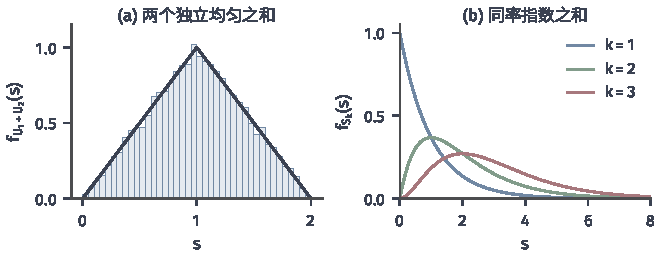
\includegraphics[width=112mm]{figures/01-basic-mathematics/05-probability-and-statistics-basics/matplotlib/rvec-convolution/figure.pdf}
  \caption{独立变量之和的密度。(a)两个独立$\operatorname{U}(0,1)$变量之和：直方图来自$20000$次模拟（固定随机种子），黑线是卷积得到的三角密度。(b)$k$个独立$\operatorname{Exp}(1)$变量之和$S_k$的密度$s^{k-1}e^{-s}/(k-1)!$，即$\operatorname{Gamma}(k,1)$；随$k$增大，峰值右移，分布变宽。}
  \label{fig:rvec-convolution}
\end{figure}

\paragraph{从Bernoulli到二项}
设$X_1,\ldots,X_n$相互独立，都服从$\operatorname{Bernoulli}(p)$，$S_n=X_1+\cdots+X_n$。对$n$归纳证明$S_n\sim\operatorname{Bin}(n,p)$。$n=1$时显然。设$S_{n-1}\sim\operatorname{Bin}(n-1,p)$；由分组独立的推论，$S_{n-1}\perp X_n$。按离散卷积，对$0\le k\le n$，
\[
\begin{aligned}
 \mathbb P(S_n=k)&=\mathbb P(S_{n-1}=k)(1-p)+\mathbb P(S_{n-1}=k-1)\,p\\
 &=\Bigl[\tbinom{n-1}{k}+\tbinom{n-1}{k-1}\Bigr]p^k(1-p)^{n-k}=\tbinom nkp^k(1-p)^{n-k},
\end{aligned}
\]
最后一步是组合数的Pascal递推，约定超出范围的组合数为零。这从卷积的角度重新得到了第~\ref{sec:prob-discrete-models}节的二项分布；独立与成功概率相同两个条件在递推的每一步都用到了。

\paragraph{从指数到Gamma}
第~\ref{sec:prob-gamma}节的$\operatorname{Gamma}(\alpha,\beta)$分布在$x>0$上的密度为$\frac{\beta^\alpha}{\Gamma(\alpha)}x^{\alpha-1}e^{-\beta x}$，$\alpha=1$时就是指数分布$\operatorname{Exp}(\beta)$。独立等待时间相加正好产生这一族分布。

\begin{theorem}[同率指数变量之和]
\label{thm:rvec-exponential-sum}
设$X_1,\ldots,X_k$相互独立，都服从$\operatorname{Exp}(\lambda)$。则$S_k=X_1+\cdots+X_k\sim\operatorname{Gamma}(k,\lambda)$，即
\[
 f_{S_k}(s)=\frac{\lambda^ks^{k-1}e^{-\lambda s}}{(k-1)!},\qquad s>0 .
\]
\end{theorem}

\begin{proof}
对$k$归纳。$k=1$时就是指数密度。设结论对$k-1$成立，$S_{k-1}\perp X_k$。两个变量都非负，卷积积分只在$0<x<s$上非零：
\[
\begin{aligned}
 f_{S_k}(s)&=\int_0^s\frac{\lambda^{k-1}x^{k-2}e^{-\lambda x}}{(k-2)!}\,\lambda e^{-\lambda(s-x)}\,\mathrm dx\\
 &=\lambda^ke^{-\lambda s}\int_0^s\frac{x^{k-2}}{(k-2)!}\,\mathrm dx=\frac{\lambda^ks^{k-1}e^{-\lambda s}}{(k-1)!} .
\end{aligned}
\]
两个指数因子合并后不再含$x$，这一步用到了两个率参数相同。
\end{proof}

例如某服务台两位顾客的服务时间独立，都服从$\operatorname{Exp}(2)$（单位：小时）。两位顾客的总服务时间超过$1$小时的概率为
\[
 \mathbb P(S_2>1)=\int_1^\infty4se^{-2s}\,\mathrm ds=3e^{-2}\approx0.406 ,
\]
而单独一位超过$1$小时的概率只有$e^{-2}\approx0.135$。图~\ref{fig:rvec-convolution}(b)画出了$\lambda=1$时$k=1,2,3$的密度。

定理的两个条件都不能省略。若率参数不同，$\lambda_1\neq\lambda_2$，同样的卷积给出$f(s)=\frac{\lambda_1\lambda_2}{\lambda_1-\lambda_2}(e^{-\lambda_2s}-e^{-\lambda_1s})$，不属于Gamma族。若不独立，例如两个“等待时间”其实是同一个$X\sim\operatorname{Exp}(\lambda)$，则$X+X=2X$满足$\mathbb P(2X>t)=e^{-\lambda t/2}$，服从$\operatorname{Exp}(\lambda/2)$，而不是$\operatorname{Gamma}(2,\lambda)$。

\subsection{乘积与比值的分布}

\paragraph{引入辅助变量}
乘积$XY$与比值$X/Y$同样是从二维到一维的映射，需要先补一个辅助变量。对乘积$W=XY$，在$x\neq0$的区域上令$(U,W)=(X,XY)$，逆映射为$(x,y)=(u,w/u)$，其Jacobian行列式为$1/u$。若$(X,Y)$有联合密度，则$\mathbb P(X=0)=0$，去掉这条直线不影响概率，于是
\[
 f_{XY}(w)=\int_{u\neq0}f_{X,Y}\Bigl(u,\frac wu\Bigr)\frac{\mathrm du}{|u|} .
\]
对比值$R=X/Y$，先检查分母：必须有$\mathbb P(Y=0)=0$，否则比值在正概率事件上没有定义。令$(R,V)=(X/Y,Y)$，逆映射为$(x,y)=(rv,v)$，行列式为$v$，得到
\[
 f_{X/Y}(r)=\int f_{X,Y}(rv,v)\,|v|\,\mathrm dv .
\]

\begin{example}[两个均匀变量的乘积]
\label{ex:rvec-uniform-product}
设$X,Y$独立，都服从$\operatorname{U}(0,1)$。被积函数在$0<u<1$且$0<w/u<1$即$w<u<1$时为$1$，故
\[
 f_{XY}(w)=\int_w^1\frac{\mathrm du}u=-\ln w,\qquad 0<w<1 .
\]
检查：$\int_0^1(-\ln w)\,\mathrm dw=1$。由此$\mathbb P(XY\le\frac12)=\int_0^{1/2}(-\ln w)\,\mathrm dw=\frac12+\frac12\ln2\approx0.847$。直接计算补事件也得到同样结果：$\mathbb P(XY>\frac12)=\int_{1/2}^1\bigl(1-\frac1{2x}\bigr)\mathrm dx=\frac12-\frac12\ln2$。
\end{example}

比值的分母可以取到零附近时，结果可能有很重的尾部。设$X,Y$独立，都服从$\mathcal N(0,1)$，则
\[
 f_{X/Y}(r)=\frac1{2\pi}\int_{-\infty}^{\infty}|v|e^{-(1+r^2)v^2/2}\,\mathrm dv=\frac1{\pi(1+r^2)} ,
\]
其中用到$\int_{-\infty}^\infty|v|e^{-av^2/2}\,\mathrm dv=2/a$。这是标准Cauchy分布。由于$\int|r|/(\pi(1+r^2))\,\mathrm dr$发散，比值的期望不存在，尽管分子和分母的各阶矩都有限。

\paragraph{由Gamma变量构造Beta变量}
第~\ref{sec:prob-beta}节的$\operatorname{Beta}(a,b)$分布在$(0,1)$上的密度为$t^{a-1}(1-t)^{b-1}/B(a,b)$，其中$B(a,b)=\int_0^1t^{a-1}(1-t)^{b-1}\,\mathrm dt$。它描述随机的比例。两段独立等待时间中第一段所占的比例，正好产生这一分布。

\begin{theorem}[Gamma变量的和与比例]
\label{thm:rvec-gamma-beta}
设$X\sim\operatorname{Gamma}(a,\beta)$，$Y\sim\operatorname{Gamma}(b,\beta)$，二者独立，率参数相同。令$S=X+Y$，$T=X/(X+Y)$。则$S\perp T$，且
\[
 S\sim\operatorname{Gamma}(a+b,\beta),\qquad T\sim\operatorname{Beta}(a,b).
\]
同时得到$B(a,b)=\Gamma(a)\Gamma(b)/\Gamma(a+b)$。
\end{theorem}

\begin{proof}
映射$(x,y)\mapsto(s,t)=(x+y,\,x/(x+y))$把$(0,\infty)^2$一一映到$(0,\infty)\times(0,1)$，逆映射为$(x,y)=(st,\,s(1-t))$，其Jacobian行列式为
\[
 \det\begin{bmatrix}t&s\\1-t&-s\end{bmatrix}=-ts-s(1-t)=-s .
\]
由独立性与定理~\ref{thm:rvec-change-of-variables}，
\[
\begin{aligned}
 f_{S,T}(s,t)&=\frac{\beta^a(st)^{a-1}e^{-\beta st}}{\Gamma(a)}\cdot\frac{\beta^b\bigl(s(1-t)\bigr)^{b-1}e^{-\beta s(1-t)}}{\Gamma(b)}\cdot s\\
 &=\frac{\beta^{a+b}s^{a+b-1}e^{-\beta s}}{\Gamma(a)\Gamma(b)}\cdot t^{a-1}(1-t)^{b-1}.
\end{aligned}
\]
两个指数因子$e^{-\beta st}e^{-\beta s(1-t)}=e^{-\beta s}$合并后不含$t$，这里用到了率参数相同。联合密度分解为$s$的函数与$t$的函数之积，取值范围是乘积形状，所以$S\perp T$。对$s$积分，由$\int_0^\infty s^{a+b-1}e^{-\beta s}\,\mathrm ds=\Gamma(a+b)/\beta^{a+b}$，
\[
 f_T(t)=\frac{\Gamma(a+b)}{\Gamma(a)\Gamma(b)}\,t^{a-1}(1-t)^{b-1},\qquad 0<t<1 .
\]
它是密度，积分为$1$，与$\operatorname{Beta}$密度的归一化比较即得$B(a,b)=\Gamma(a)\Gamma(b)/\Gamma(a+b)$。对$t$积分则得到$S$的$\operatorname{Gamma}(a+b,\beta)$密度。
\end{proof}

取$a=b=1$，$X,Y$是两个独立的$\operatorname{Exp}(\beta)$等待时间，第一段在总时间中所占比例$T$服从$\operatorname{Beta}(1,1)=\operatorname{U}(0,1)$：比例在$(0,1)$上完全均匀，与总时长无关，也与$\beta$无关。又如$a=2$、$b=3$时，$T\sim\operatorname{Beta}(2,3)$，均值为$2/5$。定理还顺带给出$S$的分布：同率独立Gamma变量之和仍是Gamma变量，形状参数相加，定理~\ref{thm:rvec-exponential-sum}是它的特例。若两个率参数不同，指数因子无法合并，$T$一般不再服从Beta分布。

\subsection{仿射变换与白化}
\label{sec:rvec-affine-whitening}

\paragraph{均值与协方差的变换}
许多组合量是分量的线性组合：多个读数的平均、两个读数之差、坐标的旋转与缩放。对这类变换，均值与协方差有简单的计算公式，不需要先求出完整分布。对两个随机向量，定义它们的\term{交叉协方差矩阵}（cross-covariance matrix）$\operatorname{Cov}(\bm X,\bm Y)=\mathbb E[(\bm X-\mathbb E\bm X)(\bm Y-\mathbb E\bm Y)^{\top}]$，其$(i,j)$元为$\operatorname{Cov}(X_i,Y_j)$。

\begin{theorem}[仿射变换的均值与协方差]
\label{thm:rvec-affine-moments}
设$\bm X\in\mathbb R^d$的均值为$\bm\mu$、协方差矩阵为$\bm\Sigma$，$\bm A\in\mathbb R^{m\times d}$，$\bm B\in\mathbb R^{k\times d}$，$\bm b\in\mathbb R^m$。则$\bm Y=\bm A\bm X+\bm b$满足
\[
 \mathbb E\bm Y=\bm A\bm\mu+\bm b,\qquad \operatorname{Cov}(\bm Y)=\bm A\bm\Sigma\bm A^{\top},\qquad
 \operatorname{Cov}(\bm A\bm X,\bm B\bm X)=\bm A\bm\Sigma\bm B^{\top}.
\]
\end{theorem}

\begin{proof}
均值公式已在第~\ref{sec:rvec-moments}节得到。由此$\bm Y-\mathbb E\bm Y=\bm A(\bm X-\bm\mu)$，故
\[
 (\bm Y-\mathbb E\bm Y)(\bm Y-\mathbb E\bm Y)^{\top}=\bm A(\bm X-\bm\mu)(\bm X-\bm\mu)^{\top}\bm A^{\top}.
\]
右端每个元素是$(\bm X-\bm\mu)(\bm X-\bm\mu)^{\top}$各元素的固定线性组合，逐元素取期望即得$\bm A\bm\Sigma\bm A^{\top}$。交叉协方差同理。
\end{proof}

公式对任意$m\times d$矩阵成立，不要求方阵，也不要求分布有密度。例如$m=1$、$\bm A=(1,1)$给出和的方差，与式~\eqref{eq:rvec-variance-of-combination}一致。求密度时则须检查维数与秩：$m=d$且$\bm A$可逆时，由定理~\ref{thm:rvec-change-of-variables}，$f_{\bm Y}(\bm y)=f_{\bm X}\bigl(\bm A^{-1}(\bm y-\bm b)\bigr)/|\det\bm A|$；$m<d$时需要补辅助变量再边缘化；$\bm A$的秩小于$m$时，$\operatorname{Cov}(\bm Y)$的秩不超过$\operatorname{rank}\bm A<m$，由第~\ref{sec:rvec-covariance-matrix}节，$\bm Y$集中在一个低维仿射子空间上，没有$m$维密度。

\begin{example}[和与差]
\label{ex:rvec-sum-difference}
设$\operatorname{Var}(X_1)=\operatorname{Var}(X_2)=1$，$\operatorname{Cov}(X_1,X_2)=0.5$。取$\bm A=\begin{bmatrix}1&1\\1&-1\end{bmatrix}$，即计算和与差：
\[
 \bm A\bm\Sigma\bm A^{\top}=\begin{bmatrix}1.5&1.5\\0.5&-0.5\end{bmatrix}\begin{bmatrix}1&1\\1&-1\end{bmatrix}=\begin{bmatrix}3&0\\0&1\end{bmatrix}.
\]
和的方差为$3$，差的方差为$1$，二者不相关。正相关使和的波动变大、差的波动变小。
\end{example}

\paragraph{白化}
上例中一个线性变换把相关的分量变成了不相关的分量。更进一步，能否找到线性变换，使结果的协方差矩阵恰好是单位矩阵？设$\bm\Sigma$正定。若矩阵$\bm W$满足$\bm W\bm\Sigma\bm W^{\top}=\bm I$，则
\[
 \bm Z=\bm W(\bm X-\bm\mu)
\]
的均值为零、协方差为$\bm I$：各分量方差为$1$，两两不相关。这样的操作称为\term{白化}（whitening）。

有两种常用的构造。第一种用Cholesky分解（式~\eqref{eq:matrix-analysis-cholesky}）$\bm\Sigma=\bm L\bm L^{\top}$，取$\bm W=\bm L^{-1}$，则$\bm L^{-1}\bm L\bm L^{\top}\bm L^{-\top}=\bm I$。第二种用谱分解（定理~\ref{thm:ls-real-symmetric-spectral}）$\bm\Sigma=\bm Q\bm\Lambda\bm Q^{\top}$，取对称平方根的逆$\bm W=\bm\Sigma^{-1/2}=\bm Q\bm\Lambda^{-1/2}\bm Q^{\top}$，矩阵平方根的计算见示例~\ref{ex:ls-matrix-square-root-two-by-two}。白化矩阵不唯一：若$\bm Z$已白化，$\bm O$是任意正交矩阵，则$\operatorname{Cov}(\bm O\bm Z)=\bm O\bm I\bm O^{\top}=\bm I$，旋转后的结果同样是白化的。

\begin{example}[用Cholesky因子白化]
\label{ex:rvec-whitening}
设$\bm\mu=(1,2)^{\top}$，$\bm\Sigma=\begin{bmatrix}4&2\\2&2\end{bmatrix}$。Cholesky因子为$\bm L=\begin{bmatrix}2&0\\1&1\end{bmatrix}$，可直接验证$\bm L\bm L^{\top}=\bm\Sigma$；其逆为$\bm L^{-1}=\begin{bmatrix}1/2&0\\-1/2&1\end{bmatrix}$。于是
\[
 Z_1=\frac{X_1-1}2,\qquad Z_2=(X_2-2)-\frac{X_1-1}2 .
\]
$Z_1$是标准化的第一个分量；$Z_2$从第二个分量中扣除了能由第一个分量线性说明的部分。验证：$\operatorname{Var}(Z_2)=2+\frac14\times4-2\times\frac12\times2=1$，$\operatorname{Cov}(Z_1,Z_2)=\frac12\times2-\frac14\times4=0$。
\end{example}

白化只保证不相关，不保证独立。图~\ref{fig:rvec-whitening}(c)中，原始样本由正方形上的均匀分布经线性变换得到，白化后协方差确实是$\bm I$，但样本均匀铺满一个倾斜的正方形：$z_1$接近正方形的左右顶点时，$z_2$只能取很窄的一段值，两个分量显然不独立。作为对照，同一协方差的高斯样本白化后，如图(b)所示呈圆形对称；第~\ref{sec:rvec-gaussian}节将说明，对联合高斯向量，白化后的分量确实相互独立。

\begin{figure}[htbp]
  \centering
  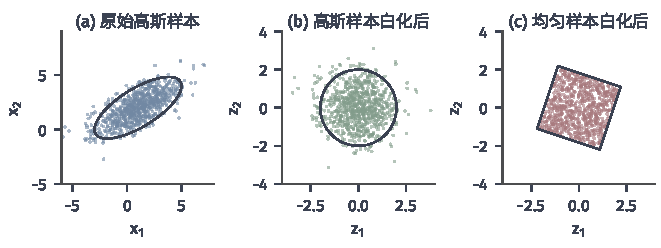
\includegraphics[width=112mm]{figures/01-basic-mathematics/05-probability-and-statistics-basics/matplotlib/rvec-whitening/figure.pdf}
  \caption{白化前后的样本，每幅$800$个模拟点（固定随机种子）。(a)均值与协方差同示例~\ref{ex:rvec-whitening}的高斯样本，椭圆是马氏距离为$2$的等密度线。(b)用Cholesky因子作变换$\bm z=\bm L^{-1}(\bm x-\bm\mu)$后，样本呈圆形对称。(c)同一协方差的非高斯样本（正方形上的均匀分布经线性变换得到）白化后，协方差同样是单位矩阵，但样本铺满一个倾斜的正方形，两个分量并不独立。}
  \label{fig:rvec-whitening}
\end{figure}

\section{随机变量的生成}
\label{sec:rvec-generation}
\label{sec:rv-random-generation}

上一节从已知分布出发计算变换后的分布。本节把问题方向转过来：给定目标分布，寻找能够产生它的随机输入和操作。模拟实验、随机算法和对模型的检验都需要这种能力。我们以第~\ref{sec:prob-continuous-models}节的标准均匀变量$U\sim\operatorname{U}(0,1)$为基本输入；计算机中的伪随机数生成器提供近似独立的均匀数，本书把它作为给定的工具。一元变量用逆变换生成，多元变量则按条件分解逐个生成；混合分布与随机参数模型是条件生成的两类具体应用。

\subsection{逆变换采样}

\paragraph{广义逆与生成定理}
第~\ref{sec:prob-numerical-features}节用分布函数的广义逆定义了分位数。对$0<u<1$，记
\[
 F^{-1}(u)=\inf\{x:F(x)\ge u\}.
\]
分布函数严格递增且连续时，它就是普通的反函数；有跳跃或平坦段时，下确界仍有定义。生成的思路是：把均匀分布的“累计概率”$u$通过分位数映回取值。

\begin{theorem}[逆变换采样]
\label{thm:rvec-inverse-transform}
设$F$是一个分布函数，$U\sim\operatorname{U}(0,1)$。则$X=F^{-1}(U)$的分布函数为$F$。
\end{theorem}

\begin{proof}
先证明：对$0<u<1$与实数$x$，$F^{-1}(u)\le x$当且仅当$u\le F(x)$。若$u\le F(x)$，则$x$属于定义下确界的集合，故$F^{-1}(u)\le x$。反过来，取该集合中趋于$F^{-1}(u)$的递减数列$x_n$，有$F(x_n)\ge u$；由分布函数的右连续性，$F\bigl(F^{-1}(u)\bigr)\ge u$。若$F^{-1}(u)\le x$，由单调性$F(x)\ge F\bigl(F^{-1}(u)\bigr)\ge u$。于是
\[
 \mathbb P(X\le x)=\mathbb P\bigl(F^{-1}(U)\le x\bigr)=\mathbb P\bigl(U\le F(x)\bigr)=F(x).
\]
\end{proof}

这种方法称为\term{逆变换采样}（inverse transform sampling）。图~\ref{fig:rvec-inverse-transform}给出了它的几何读法：在纵轴上取均匀点$u$，向右作水平线，碰到分布函数图像（或跳跃的竖直缺口）后向下投影，落点就是生成值。分布函数陡峭的地方，一段纵轴高度只对应很短的横轴区间，生成值在那里密集；平坦的地方则相反。

\begin{figure}[htbp]
  \centering
  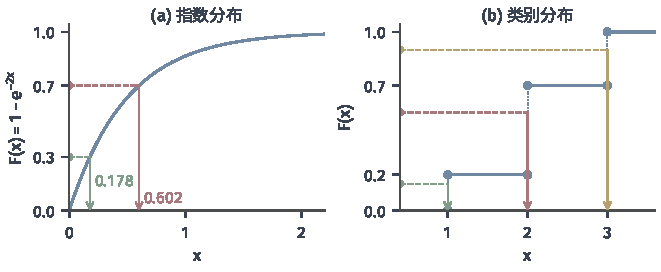
\includegraphics[width=112mm]{figures/01-basic-mathematics/05-probability-and-statistics-basics/matplotlib/rvec-inverse-transform/figure.pdf}
  \caption{逆变换采样的几何读法。(a)指数分布$\operatorname{Exp}(2)$：纵轴上的$u=0.3$和$u=0.7$经分布函数映回$x\approx0.178$和$x\approx0.602$。(b)在$1,2,3$上概率为$0.2,0.5,0.3$的类别分布：分布函数是阶梯，纵轴区间$(0,0.2]$、$(0.2,0.7]$、$(0.7,1]$分别映到$1$、$2$、$3$，图中$u=0.15,0.55,0.9$各落入一个区间。}
  \label{fig:rvec-inverse-transform}
\end{figure}

\paragraph{离散与连续两个例子}
定理不要求分布函数连续或严格递增，所以离散分布同样适用。设$X$在$\{1,2,3\}$上的概率为$0.2,0.5,0.3$，累计值为$c_1=0.2$、$c_2=0.7$、$c_3=1$。广义逆在$(0,0.2]$上取$1$，在$(0.2,0.7]$上取$2$，在$(0.7,1)$上取$3$，于是生成规则是“$U$落入第$k$段就输出$k$”，第$k$段的长度恰为$\pi_k$。分布函数的每一次跳跃把一整段$u$映到同一个取值；分布函数的平坦段（例如$1$与$2$之间）对应概率为零的区间，不会被生成。

对指数分布$\operatorname{Exp}(\lambda)$，$F(x)=1-e^{-\lambda x}$在$x>0$上连续递增，解$1-e^{-\lambda x}=u$得
\[
 F^{-1}(u)=-\frac{\ln(1-u)}\lambda .
\]
$\lambda=2$时，$u=0.3$生成$-\ln0.7/2\approx0.178$，$u=0.7$生成$-\ln0.3/2\approx0.602$。由于$1-U$与$U$同分布，也可以直接用$-\ln U/\lambda$。

\paragraph{用组合变换生成高斯变量}
逆变换采样需要能计算$F^{-1}$。标准高斯分布函数$\Phi$没有初等形式的反函数，此时可以把第~\ref{sec:rvec-transforms}节的变换倒过来使用。

\begin{example}[Box--Muller方法]
\label{ex:rvec-box-muller}
取独立的$U_1,U_2\sim\operatorname{U}(0,1)$，令
\[
 R=\sqrt{-2\ln U_1},\qquad \Theta=2\pi U_2,\qquad (X,Y)=(R\cos\Theta,\,R\sin\Theta).
\]
由逆变换采样，$-\ln U_1\sim\operatorname{Exp}(1)$，所以$R^2/2\sim\operatorname{Exp}(1)$，$R$的密度为$re^{-r^2/2}$；$\Theta\sim\operatorname{U}(0,2\pi)$且与$R$独立。这正是示例~\ref{ex:rvec-polar-gaussian}中$(R,\Theta)$的联合分布。把那里的极坐标变换反过来用一次定理~\ref{thm:rvec-change-of-variables}，即知$X,Y$是两个独立的标准高斯变量。
\end{example}

\subsection{条件生成}

\paragraph{按条件分解逐个生成}
多元变量可以拆成一连串一元问题。第~\ref{sec:rvec-conditioning}节的乘积关系$p_{X,Y}(x,y)=p_X(x)\,p_{Y\mid X}(y\mid x)$提示了生成顺序：先按$p_X$生成$X$，得到取值$x$以后，再用新的、独立的随机输入按条件分布$p_{Y\mid X}(\cdot\mid x)$生成$Y$。这样得到的一对$(X,Y)$满足
\[
\begin{aligned}
 \mathbb P(X=x,Y=y)&=\mathbb P(X=x)\,\mathbb P(Y=y\mid X=x)\\
 &=p_X(x)\,p_{Y\mid X}(y\mid x)=p_{X,Y}(x,y),
\end{aligned}
\]
恰好是目标联合分布；密度情形同理。$d$个变量时，反复使用乘法公式得到
\[
 p(x_1,\ldots,x_d)=p(x_1)\,p(x_2\mid x_1)\cdots p(x_d\mid x_1,\ldots,x_{d-1}),
\]
按这个顺序逐个生成即可。例如示例~\ref{ex:rvec-study-table}的概率表可以这样生成：先以概率$0.3,0.4,0.3$抽取$X\in\{0,1,2\}$，再按$\operatorname{Bernoulli}(m(X))$抽取$Y$，其中$m=(1/3,5/8,5/6)$。核对一格：$\mathbb P(X=2,Y=1)=0.3\times5/6=0.25$。

\paragraph{有限混合}
若观测来自几个未加标记的来源，例如两条产线的产品混在一起，可以先抽取来源标签，再按该来源的分布生成观测。设$Z\sim\operatorname{Cat}(\bm w)$取值$1,\ldots,K$，权重$w_k>0$且和为$1$；给定$Z=k$时，$X$的密度为$f_k$。由全概率公式，$\mathbb P(X\le x)=\sum_kw_k\,\mathbb P(X\le x\mid Z=k)$，求导得到
\[
 f_X(x)=\sum_{k=1}^Kw_kf_k(x).
\]
这样的分布称为\term{混合分布}（mixture distribution）。标签$Z$在观测中不出现，是一个\term{潜变量}（latent variable）；它不必对应真实可辨认的类别，主要用于组织模型与计算。

\begin{example}[两个高斯分量的混合]
\label{ex:rvec-gaussian-mixture}
取$\bm w=(1/4,3/4)$，$X\mid Z=1\sim\mathcal N(-1,1)$，$X\mid Z=2\sim\mathcal N(1,1)$。由全期望公式，$\mathbb EX=\frac14\times(-1)+\frac34\times1=\frac12$。由全方差公式，组内部分为$1$，组间部分为$\frac14\times1+\frac34\times1-\frac14=\frac34$，所以$\operatorname{Var}(X)=\frac74$；只平均两个分量的方差会漏掉均值不同造成的$3/4$。图~\ref{fig:rvec-gaussian-mixture}比较了两步生成的样本与混合密度：密度只有一个峰，但左侧明显比单个高斯更厚，这是权重较小的左分量的贡献。
\end{example}

\begin{figure}[htbp]
  \centering
  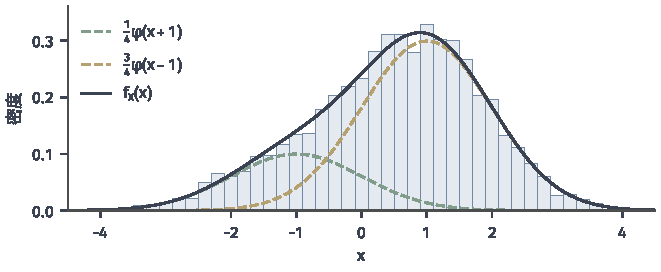
\includegraphics[width=112mm]{figures/01-basic-mathematics/05-probability-and-statistics-basics/matplotlib/rvec-mixture/figure.pdf}
  \caption{两个高斯分量的混合。先以概率$1/4,3/4$抽取标签，再从$\mathcal N(-1,1)$或$\mathcal N(1,1)$生成观测；直方图来自$4000$次两步生成（固定随机种子）。两条虚线是加权后的分量密度，黑线是它们的和$f_X$，其中$\varphi$为标准高斯密度。}
  \label{fig:rvec-gaussian-mixture}
\end{figure}

反过来，观测到$X=x$以后，可以用Bayes公式推断它来自哪个分量：
\[
 \mathbb P(Z=k\mid X=x)=\frac{w_kf_k(x)}{\sum_jw_jf_j(x)} .
\]
这里条件变量$Z$离散、观测$X$有密度，公式可以像条件密度那样由窄带$\{x\le X\le x+h\}$上的条件概率取极限得到。在上例中，$x=0$处两个分量密度相等，后验概率就等于权重$(1/4,3/4)$；$x=1$处，$\mathbb P(Z=1\mid X=1)=\frac{\frac14e^{-2}}{\frac14e^{-2}+\frac34}\approx0.043$。

\paragraph{随机参数模型}
另一类常见的条件生成是先生成参数，再在参数给定时生成多个观测。设参数$\Theta$有密度$f_\Theta$，给定$\Theta=\theta$时，$X_1,\ldots,X_n$条件独立，各自服从由$\theta$决定的同一分布$p(\cdot\mid\theta)$。联合分布为
\[
 f_\Theta(\theta)\prod_{i=1}^np(x_i\mid\theta),
\]
生成时先抽$\Theta$，再用这个取值独立地抽出$n$个观测。这样的分层构造称为\term{层次模型}（hierarchical model）。第~\ref{sec:rvec-conditioning}节的两枚硬币例子是参数只取两个值的情形；下面让参数在$(0,1)$上连续变化。

\begin{example}[Beta--Bernoulli模型]
\label{ex:rvec-beta-bernoulli}
设$\Theta\sim\operatorname{Beta}(a,b)$，给定$\Theta=\theta$时$X_1,\ldots,X_n$条件独立，都服从$\operatorname{Bernoulli}(\theta)$。可以把$\Theta$理解为某个未知的成功率，$X_i$为各次试验的结果。对观测序列$x_1,\ldots,x_n\in\{0,1\}$，记成功次数$k=\sum_ix_i$。把全概率公式中的求和换成对参数的积分，
\[
\begin{aligned}
 \mathbb P(X_1=x_1,\ldots,X_n=x_n)&=\int_0^1\theta^k(1-\theta)^{n-k}\frac{\theta^{a-1}(1-\theta)^{b-1}}{B(a,b)}\,\mathrm d\theta\\
 &=\frac{B(a+k,\,b+n-k)}{B(a,b)} .
\end{aligned}
\]
它只依赖成功次数$k$，不依赖成功出现的顺序。

用条件期望计算依赖强度更直接。给定$\Theta$，$\mathbb E[X_1\mid\Theta]=\Theta$；由条件独立，$\mathbb E[X_1X_2\mid\Theta]=\Theta^2$。由全期望公式，
\[
\begin{gathered}
 \mathbb P(X_1=1)=\mathbb E\Theta,\qquad \mathbb E[X_1X_2]=\mathbb E\Theta^2,\\
 \operatorname{Cov}(X_1,X_2)=\mathbb E\Theta^2-(\mathbb E\Theta)^2=\operatorname{Var}(\Theta)>0 .
\end{gathered}
\]
由第~\ref{sec:prob-beta}节，$\mathbb E\Theta=a/(a+b)$，$\operatorname{Var}(\Theta)=ab/\bigl((a+b)^2(a+b+1)\bigr)$。又$\operatorname{Var}(X_1)=\mathbb E\Theta(1-\mathbb E\Theta)=ab/(a+b)^2$，所以
\[
 \operatorname{Corr}(X_1,X_2)=\frac1{a+b+1} .
\]
$a=b=1$时$\Theta$在$(0,1)$上均匀，$\mathbb P(X_1=1)=1/2$，$\mathbb P(X_1=1,X_2=1)=\mathbb E\Theta^2=1/3$，于是$\mathbb P(X_2=1\mid X_1=1)=2/3$，相关系数为$1/3$。$a=b=10$时$\Theta$集中在$1/2$附近，相关系数降为$1/21\approx0.048$。
\end{example}

这个例子说明了共享参数产生依赖的机制：给定参数时观测条件独立，但参数未知时，每个观测都携带关于参数的信息，进而影响对其他观测的预测。参数越不确定（$\operatorname{Var}(\Theta)$越大），观测之间的边缘依赖越强；参数完全确定时，依赖消失。由观测更新$\Theta$的分布是第~\ref{sec:est-posterior}节的后验计算，据此预测下一次结果则在第~\ref{sec:pred-prediction}节讨论；本节只关心模型怎样生成数据以及由此产生的依赖结构。

\section{多元高斯分布}
\label{sec:rvec-gaussian}

前面各节分别建立了联合与边缘分布、协方差、独立与条件分布、变换与生成。本节集中研究一个模型，在其中把这些操作全部做一遍。多元高斯分布由均值向量和协方差矩阵完全确定，上述每一种操作都能在这两个参数上直接完成。

\subsection{多元高斯分布的定义}

\paragraph{密度与等密度椭球}
第~\ref{sec:prob-gaussian}节的一元高斯密度在指数中含有$(x-\mu)^2/\sigma^2$，即偏离量按方差标准化后的平方。多元情形中偏离是一个向量，自然的推广是用协方差矩阵的逆构造二次型。

\begin{definition}[多元高斯分布]
设$\bm\mu\in\mathbb R^d$，$\bm\Sigma$是$d\times d$对称正定矩阵。若随机向量$\bm X$的联合密度为
\begin{equation}
 f_{\bm X}(\bm x)=\frac1{(2\pi)^{d/2}(\det\bm\Sigma)^{1/2}}
 \exp\Bigl\{-\frac12(\bm x-\bm\mu)^{\top}\bm\Sigma^{-1}(\bm x-\bm\mu)\Bigr\},\qquad\bm x\in\mathbb R^d,
 \label{eq:rvec-gaussian-density}
\end{equation}
则称$\bm X$服从参数为$\bm\mu,\bm\Sigma$的\term{多元高斯分布}（multivariate Gaussian distribution），记为$\bm X\sim\mathcal N(\bm\mu,\bm\Sigma)$。
\end{definition}

$d=1$时它回到一元高斯密度。下一小节将验证这个函数积分为$1$，且$\bm\mu$与$\bm\Sigma$正是$\bm X$的均值向量与协方差矩阵。若$\bm\Sigma$是对角矩阵，二次型分解为$\sum_i(x_i-\mu_i)^2/\sigma_i^2$，密度变成$d$个一元高斯密度之积，各分量相互独立。

密度只通过二次型$Q(\bm x)=(\bm x-\bm\mu)^{\top}\bm\Sigma^{-1}(\bm x-\bm\mu)$依赖$\bm x$，所以等密度集合是$Q(\bm x)=c^2$。用谱分解$\bm\Sigma=\sum_i\lambda_i\bm q_i\bm q_i^{\top}$，在以$\bm\mu$为原点、以特征向量$\bm q_i$为坐标轴的坐标$u_i=\bm q_i^{\top}(\bm x-\bm\mu)$下，$Q=\sum_iu_i^2/\lambda_i$。因此等密度集合是以$\bm\mu$为中心的椭球，主轴沿特征向量方向，半轴长为$c\sqrt{\lambda_i}$：方差大的方向上椭球更长。$\sqrt{Q(\bm x)}$称为$\bm x$到$\bm\mu$的\term{马氏距离}（Mahalanobis distance），它按各方向的波动大小度量偏离。

\begin{example}[一个二维高斯分布]
\label{ex:rvec-gaussian-2d}
本节始终使用示例~\ref{ex:rvec-whitening}的参数$\bm\mu=(1,2)^{\top}$，$\bm\Sigma=\begin{bmatrix}4&2\\2&2\end{bmatrix}$。此时$\det\bm\Sigma=4$，
\[
 \bm\Sigma^{-1}=\begin{bmatrix}1/2&-1/2\\-1/2&1\end{bmatrix},\qquad
 Q(\bm x)=\tfrac12u_1^2-u_1u_2+u_2^2,\quad \bm u=\bm x-\bm\mu .
\]
特征值为$3\pm\sqrt5$，约为$5.24$与$0.76$。长轴方向的特征向量满足$(4-\lambda)v_1+2v_2=0$，取$\lambda=3+\sqrt5$得斜率$v_2/v_1=(\sqrt5-1)/2\approx0.62$。图~\ref{fig:rvec-gaussian-conditional}(a)画出了$c=1,2,3$的等密度椭圆：它们向右上方倾斜，反映两个分量正相关，相关系数为$2/\sqrt{4\times2}\approx0.71$。
\end{example}

\paragraph{分量高斯不等于联合高斯}
联合高斯是整个向量的性质，不能由每个分量的分布判断。示例~\ref{ex:rvec-random-sign}的$(Z,SZ)$两个分量都服从$\mathcal N(0,1)$，但它们不是联合高斯：散点全部落在两条对角线上，面积为零，没有二维联合密度。下一小节将证明，联合高斯向量的任何非零线性组合都服从一元高斯分布；而$Z+SZ$在$S=-1$时等于零，$\mathbb P(Z+SZ=0)=1/2$，一个正方差的高斯变量取任何单点的概率都是零。因此，即使每个分量都是高斯变量，向量整体也可能不是多元高斯分布。

\subsection{仿射变换与生成}

\paragraph{由独立标准高斯变量生成}
最简单的多元高斯向量由独立的标准高斯变量排成。设$Z_1,\ldots,Z_d$相互独立，都服从$\mathcal N(0,1)$，则$\bm Z=(Z_1,\ldots,Z_d)^{\top}$的联合密度为
\[
 \prod_{i=1}^d\frac1{\sqrt{2\pi}}e^{-z_i^2/2}=\frac1{(2\pi)^{d/2}}e^{-\bm z^{\top}\bm z/2},
\]
正是式~\eqref{eq:rvec-gaussian-density}取$\bm\mu=\bm0$、$\bm\Sigma=\bm I$的情形，即$\bm Z\sim\mathcal N(\bm0,\bm I)$。一般的高斯向量可以由它经可逆仿射变换得到。

\begin{theorem}[多元高斯向量的生成]
\label{thm:rvec-gaussian-generation}
设$\bm Z\sim\mathcal N(\bm0,\bm I_d)$，$\bm A$是$d\times d$可逆矩阵，$\bm A\bm A^{\top}=\bm\Sigma$。则$\bm X=\bm\mu+\bm A\bm Z\sim\mathcal N(\bm\mu,\bm\Sigma)$。特别地，式~\eqref{eq:rvec-gaussian-density}积分为$1$，且$\mathbb E\bm X=\bm\mu$，$\operatorname{Cov}(\bm X)=\bm\Sigma$。
\end{theorem}

\begin{proof}
映射$\bm z\mapsto\bm\mu+\bm A\bm z$可逆，逆映射为$\bm z=\bm A^{-1}(\bm x-\bm\mu)$，其Jacobian行列式为$\det\bm A^{-1}$。由$\det\bm\Sigma=(\det\bm A)^2$，$|\det\bm A^{-1}|=(\det\bm\Sigma)^{-1/2}$。又
\[
 \bm z^{\top}\bm z=(\bm x-\bm\mu)^{\top}\bm A^{-\top}\bm A^{-1}(\bm x-\bm\mu)=(\bm x-\bm\mu)^{\top}\bm\Sigma^{-1}(\bm x-\bm\mu),
\]
因为$\bm A^{-\top}\bm A^{-1}=(\bm A\bm A^{\top})^{-1}$。代入定理~\ref{thm:rvec-change-of-variables}，$\bm X$的密度正是式~\eqref{eq:rvec-gaussian-density}。它是一个随机向量的密度，积分自然为$1$。由定理~\ref{thm:rvec-affine-moments}，$\mathbb E\bm X=\bm\mu$，$\operatorname{Cov}(\bm X)=\bm A\bm I\bm A^{\top}=\bm\Sigma$。
\end{proof}

满足$\bm A\bm A^{\top}=\bm\Sigma$的矩阵可取Cholesky因子$\bm L$，也可取对称平方根$\bm\Sigma^{1/2}$。于是生成$\mathcal N(\bm\mu,\bm\Sigma)$的步骤是：分解$\bm\Sigma=\bm L\bm L^{\top}$；生成$d$个独立标准高斯数组成$\bm z$（例如用Box--Muller方法）；输出$\bm x=\bm\mu+\bm L\bm z$。这正是白化的逆过程。对示例~\ref{ex:rvec-gaussian-2d}，$\bm L=\begin{bmatrix}2&0\\1&1\end{bmatrix}$，
\[
 X_1=1+2Z_1,\qquad X_2=2+Z_1+Z_2 .
\]
例如$\bm z=(0.5,-1)^{\top}$生成$\bm x=(2,1.5)^{\top}$。两个分量共享$Z_1$，这就是它们正相关的来源：$\operatorname{Cov}(X_1,X_2)=2\operatorname{Var}(Z_1)=2$。

\paragraph{仿射变换保持高斯结构}
高斯向量经过线性变换后仍是高斯向量，这是这一模型便于计算的根本原因。

\begin{theorem}[仿射变换]
\label{thm:rvec-gaussian-affine}
设$\bm X\sim\mathcal N(\bm\mu,\bm\Sigma)$，$\bm B$是秩为$m$的$m\times d$矩阵，$\bm c\in\mathbb R^m$。则
\[
 \bm B\bm X+\bm c\sim\mathcal N\bigl(\bm B\bm\mu+\bm c,\;\bm B\bm\Sigma\bm B^{\top}\bigr).
\]
特别地，对任意$\bm a\neq\bm0$，$\bm a^{\top}\bm X\sim\mathcal N(\bm a^{\top}\bm\mu,\bm a^{\top}\bm\Sigma\bm a)$。
\end{theorem}

\begin{proof}
由定理~\ref{thm:rvec-gaussian-generation}，可写$\bm X=\bm\mu+\bm L\bm Z$，于是$\bm B\bm X+\bm c=\bm B\bm\mu+\bm c+\bm M\bm Z$，其中$\bm M=\bm B\bm L$的秩为$m$，$\bm M\bm M^{\top}=\bm B\bm\Sigma\bm B^{\top}$正定。只需证明$\bm M\bm Z\sim\mathcal N(\bm0,\bm M\bm M^{\top})$。

令$\bm K=(\bm M\bm M^{\top})^{-1/2}\bm M$，其中逆平方根由谱分解给出。则$\bm K\bm K^{\top}=\bm I_m$，即$\bm K$的$m$行是标准正交的。用Gram--Schmidt正交化（第~\ref{chap:normed-inner-product-spaces}章）把这些行补成$\mathbb R^d$的标准正交基，排成正交矩阵$\bm O=\begin{bmatrix}\bm K\\\bm K'\end{bmatrix}$。由定理~\ref{thm:rvec-gaussian-generation}（取$\bm A=\bm O$，$\bm O\bm O^{\top}=\bm I$），$\bm O\bm Z\sim\mathcal N(\bm0,\bm I_d)$，即$\bm O\bm Z$的$d$个分量是独立的标准高斯变量。它的前$m$个分量$\bm K\bm Z$的联合密度由乘积密度对其余分量积分得到，各因子积分为$1$，所以$\bm K\bm Z\sim\mathcal N(\bm0,\bm I_m)$。最后$\bm M\bm Z=(\bm M\bm M^{\top})^{1/2}\bm K\bm Z$，再用一次定理~\ref{thm:rvec-gaussian-generation}即得结论。
\end{proof}

对示例~\ref{ex:rvec-gaussian-2d}，$X_1+X_2\sim\mathcal N(3,\,4+2\times2+2)=\mathcal N(3,10)$。又取$\bm a=(-1/2,1)^{\top}$，$\bm a^{\top}\bm\Sigma\bm a=\frac14\times4-2\times\frac12\times2+2=1$，故$X_2-X_1/2\sim\mathcal N(3/2,1)$；它减去均值就是示例~\ref{ex:rvec-whitening}中的$Z_2$。

\paragraph{退化高斯分布}
若矩阵的秩不足，结论需要修改。例如取$\bm B=\begin{bmatrix}1&1\\2&2\end{bmatrix}$，$\bm B\bm X=(S,2S)^{\top}$，其中$S=X_1+X_2\sim\mathcal N(3,10)$。这个二维向量全部落在直线$y=2x$上，没有二维密度，$\bm B\bm\Sigma\bm B^{\top}$也是奇异的。更一般地，对任意矩阵$\bm M$（不论秩），称$\bm c+\bm M\bm Z$的分布为（可能）\term{退化高斯分布}（degenerate Gaussian distribution），其均值为$\bm c$、协方差为$\bm M\bm M^{\top}$。秩不足时概率集中在仿射子空间$\bm c+\operatorname{range}(\bm M)$上，在这个子空间内的坐标下仍是非退化的高斯分布。这个分布只取决于$\bm c$与$\bm M\bm M^{\top}$，而不取决于$\bm M$本身的选取；证明需要特征函数，留到\BookPartRef{part:probability-spaces}{卷2《数学准备：抽象数学》的“概率空间”部分}。有了这一推广，定理~\ref{thm:rvec-gaussian-affine}对任意$\bm B$都成立，只是结果可能退化。

\subsection{边缘分布}

\paragraph{取出部分分量}
取出部分分量是一个特殊的线性映射。设$\bm X\sim\mathcal N(\bm\mu,\bm\Sigma)$，要保留前$k$个分量$\bm X_1=(X_1,\ldots,X_k)^{\top}$，取$\bm B=[\bm I_k\ \bm0]$，它的秩为$k$。由定理~\ref{thm:rvec-gaussian-affine}，
\[
 \bm X_1\sim\mathcal N(\bm\mu_1,\bm\Sigma_{11}),
\]
其中$\bm\mu_1$是$\bm\mu$的前$k$个分量，$\bm\Sigma_{11}$是$\bm\Sigma$左上角的$k\times k$子矩阵。保留任意一组分量时，选出$\bm I_d$的相应行即可。高斯分布的边缘化因此不需要计算积分，只需从参数中取出相应的子向量和子矩阵。示例~\ref{ex:rvec-gaussian-2d}中，$X_1\sim\mathcal N(1,4)$，$X_2\sim\mathcal N(2,2)$。

\paragraph{分块记号}
为了讨论两组分量之间的关系，把向量与参数按相同方式分块：
\[
 \bm X=\begin{bmatrix}\bm X_1\\\bm X_2\end{bmatrix},\qquad
 \bm\mu=\begin{bmatrix}\bm\mu_1\\\bm\mu_2\end{bmatrix},\qquad
 \bm\Sigma=\begin{bmatrix}\bm\Sigma_{11}&\bm\Sigma_{12}\\\bm\Sigma_{21}&\bm\Sigma_{22}\end{bmatrix},
\]
其中$\bm\Sigma_{12}=\operatorname{Cov}(\bm X_1,\bm X_2)$是两块之间的交叉协方差矩阵，$\bm\Sigma_{21}=\bm\Sigma_{12}^{\top}$。两个边缘分布只用到对角块$\bm\mu_1,\bm\Sigma_{11}$与$\bm\mu_2,\bm\Sigma_{22}$；两组分量之间的联系全部记录在$\bm\Sigma_{12}$中。例如把示例~\ref{ex:rvec-gaussian-2d}的非对角元由$2$改为$0$或$-1$，两个边缘分布不变，联合分布却不同。下面两小节分别回答：$\bm\Sigma_{12}=\bm0$意味着什么，以及观测到$\bm X_2$以后$\bm X_1$的分布怎样计算。

\subsection{独立性}

\paragraph{零交叉协方差推出独立}
第~\ref{sec:rvec-independence}节说明不相关一般推不出独立。联合高斯模型是一个重要例外。这里两个随机向量的独立按第~\ref{sec:rvec-independence}节的定义理解，只是把$A,B$换成相应维数空间中的集合；密度判定照样成立。

\begin{theorem}[联合高斯向量的分块独立]
\label{thm:rvec-gaussian-independence}
设$\bm X\sim\mathcal N(\bm\mu,\bm\Sigma)$按上述方式分块。若$\bm\Sigma_{12}=\bm0$，则$\bm X_1\perp\bm X_2$。
\end{theorem}

\begin{proof}
$\bm\Sigma_{12}=\bm0$时$\bm\Sigma$是分块对角矩阵，于是
\[
 \bm\Sigma^{-1}=\begin{bmatrix}\bm\Sigma_{11}^{-1}&\bm0\\\bm0&\bm\Sigma_{22}^{-1}\end{bmatrix},\qquad
 \det\bm\Sigma=\det\bm\Sigma_{11}\det\bm\Sigma_{22},
\]
二次型分成两项：$(\bm x-\bm\mu)^{\top}\bm\Sigma^{-1}(\bm x-\bm\mu)=(\bm x_1-\bm\mu_1)^{\top}\bm\Sigma_{11}^{-1}(\bm x_1-\bm\mu_1)+(\bm x_2-\bm\mu_2)^{\top}\bm\Sigma_{22}^{-1}(\bm x_2-\bm\mu_2)$。常数因子$(2\pi)^{d/2}$也按维数拆开。因此式~\eqref{eq:rvec-gaussian-density}等于$\mathcal N(\bm\mu_1,\bm\Sigma_{11})$与$\mathcal N(\bm\mu_2,\bm\Sigma_{22})$两个密度之积，而它们正是两块的边缘密度。由独立性的密度判定，$\bm X_1\perp\bm X_2$。
\end{proof}

逐个分量地应用：若$\bm\Sigma$是对角矩阵，联合高斯向量的各分量相互独立。定理的条件是整个向量联合高斯，而不只是各分量高斯。示例~\ref{ex:rvec-random-sign}中$\operatorname{Cov}(Z,SZ)=\mathbb E[S]\,\mathbb E[Z^2]=0$，两个分量都是标准高斯变量，却并不独立；它们不是联合高斯，定理不适用。

\paragraph{白化后的独立性}
回到第~\ref{sec:rvec-affine-whitening}节的白化。若$\bm X\sim\mathcal N(\bm\mu,\bm\Sigma)$，则由定理~\ref{thm:rvec-gaussian-affine}，$\bm Z=\bm L^{-1}(\bm X-\bm\mu)\sim\mathcal N(\bm0,\bm I)$。协方差为单位矩阵，由上面的定理，$\bm Z$的分量是相互独立的标准高斯变量。对一般分布，白化只能保证不相关；对联合高斯向量，白化把分量变成了独立变量，图~\ref{fig:rvec-whitening}(b)与(c)的差别正在于此。又因为$\mathcal N(\bm0,\bm I)$经任意正交变换仍是$\mathcal N(\bm0,\bm I)$，高斯情形下白化矩阵的不唯一性不影响这个结论。

\subsection{条件分布}
\label{sec:rvec-gaussian-conditioning}

\paragraph{条件均值与条件协方差}
观测到一部分分量以后，其余分量的分布应当怎样计算？对联合高斯向量，答案仍是高斯分布，参数可以由分块协方差直接写出。思路是把$\bm X_1$拆成“由$\bm X_2$线性决定的部分”与“和$\bm X_2$独立的残差”。

\begin{theorem}[高斯条件分布]
\label{thm:rvec-gaussian-conditional}
设$\bm X\sim\mathcal N(\bm\mu,\bm\Sigma)$按上述方式分块。对任意$\bm x_2$，
\begin{equation}
 \bm X_1\mid\bm X_2=\bm x_2\ \sim\ \mathcal N\Bigl(\bm\mu_1+\bm\Sigma_{12}\bm\Sigma_{22}^{-1}(\bm x_2-\bm\mu_2),\ \ \bm\Sigma_{11}-\bm\Sigma_{12}\bm\Sigma_{22}^{-1}\bm\Sigma_{21}\Bigr).
 \label{eq:rvec-gaussian-conditional}
\end{equation}
\end{theorem}

\begin{proof}
记$\bm K=\bm\Sigma_{12}\bm\Sigma_{22}^{-1}$（$\bm\Sigma_{22}$作为正定矩阵的主子矩阵是正定的，因而可逆），令残差
\[
 \bm R=\bm X_1-\bm\mu_1-\bm K(\bm X_2-\bm\mu_2).
\]
向量$(\bm R,\bm X_2)$由$\bm X$经可逆仿射变换得到，变换矩阵$\begin{bmatrix}\bm I&-\bm K\\\bm0&\bm I\end{bmatrix}$是行列式为$1$的分块三角矩阵，所以$(\bm R,\bm X_2)$联合高斯。由定理~\ref{thm:rvec-affine-moments}，
\[
\begin{aligned}
 \operatorname{Cov}(\bm R,\bm X_2)&=\bm\Sigma_{12}-\bm K\bm\Sigma_{22}=\bm0,\\
 \operatorname{Cov}(\bm R)&=\bm\Sigma_{11}-\bm K\bm\Sigma_{21}-\bm\Sigma_{12}\bm K^{\top}+\bm K\bm\Sigma_{22}\bm K^{\top}\\
 &=\bm\Sigma_{11}-\bm\Sigma_{12}\bm\Sigma_{22}^{-1}\bm\Sigma_{21},
\end{aligned}
\]
后一式中三项$\bm K\bm\Sigma_{21}$、$\bm\Sigma_{12}\bm K^{\top}$、$\bm K\bm\Sigma_{22}\bm K^{\top}$都等于$\bm\Sigma_{12}\bm\Sigma_{22}^{-1}\bm\Sigma_{21}$。记这个矩阵为$\bm S$。$(\bm R,\bm X_2)$的协方差矩阵是正定矩阵经可逆合同变换的结果，仍正定，所以其对角块$\bm S$正定。由定理~\ref{thm:rvec-gaussian-independence}，$\bm R\perp\bm X_2$，且$\bm R\sim\mathcal N(\bm0,\bm S)$。

记$m(\bm x_2)=\bm\mu_1+\bm K(\bm x_2-\bm\mu_2)$。对$(\bm x_1,\bm x_2)\mapsto(\bm x_1-m(\bm x_2),\bm x_2)$用定理~\ref{thm:rvec-change-of-variables}（行列式为$1$），并利用独立性，
\[
 f_{\bm X_1,\bm X_2}(\bm x_1,\bm x_2)=f_{\bm R,\bm X_2}\bigl(\bm x_1-m(\bm x_2),\bm x_2\bigr)=f_{\bm R}\bigl(\bm x_1-m(\bm x_2)\bigr)f_{\bm X_2}(\bm x_2).
\]
除以$f_{\bm X_2}(\bm x_2)>0$，条件密度为$f_{\bm R}\bigl(\bm x_1-m(\bm x_2)\bigr)$，即$\mathcal N\bigl(m(\bm x_2),\bm S\bigr)$的密度。
\end{proof}

条件协方差$\bm S=\bm\Sigma_{11}-\bm\Sigma_{12}\bm\Sigma_{22}^{-1}\bm\Sigma_{21}$正是$\bm\Sigma$中对块$\bm\Sigma_{22}$的Schur补；式~\eqref{eq:matrix-analysis-schur-positive-definite}说明了它为何正定。从协方差的角度看，它是从$\bm X_1$的原有波动$\bm\Sigma_{11}$中扣除能由$\bm X_2$线性说明的部分后剩下的波动。对联合密度的指数直接配方，借助分块逆公式~\eqref{eq:matrix-analysis-block-inverse}，也能得到同样的结果；上面的残差证明则说明了结果的含义。条件均值是$\bm x_2$的仿射函数，条件协方差则完全不依赖观测值$\bm x_2$：残差与$\bm X_2$独立，观测只移动中心，不改变围绕中心的波动。

\paragraph{二维算例}
对示例~\ref{ex:rvec-gaussian-2d}，以$X_1$为观测分量、求$X_2$的条件分布，把公式中两块的角色互换：
\[
\begin{aligned}
 \mathbb E[X_2\mid X_1=x_1]&=2+\frac24(x_1-1)=2+\frac{x_1-1}2,\\
 \operatorname{Var}(X_2\mid X_1=x_1)&=2-\frac{2\times2}4=1 .
\end{aligned}
\]
观测到$X_1=5$时，$X_2\mid X_1=5\sim\mathcal N(4,1)$。观测之前，$X_2\sim\mathcal N(2,2)$，$\mathbb P(X_2>3)=1-\Phi(1/\sqrt2)\approx0.240$；观测之后，$\mathbb P(X_2>3\mid X_1=5)=1-\Phi(-1)\approx0.841$。观测把预测中心从$2$移到$4$，把方差从$2$缩小到$1$。

图~\ref{fig:rvec-gaussian-conditional}显示了这个过程。在(a)中，竖直虚线$x_1=5$切过等密度椭圆，切片上的密度经归一化就是条件密度；红线是条件均值$m(x_1)$，它经过均值点$(1,2)$，斜率为$1/2$。(b)比较了观测前后$X_2$的密度。这个计算与Cholesky生成过程一致：由$X_1=1+2Z_1$得$Z_1=(X_1-1)/2$，代入$X_2=2+Z_1+Z_2$，得到$X_2=m(X_1)+Z_2$；残差正是与$X_1$独立的$Z_2$，所以无论观测到的$x_1$是多少，条件方差都是$\operatorname{Var}(Z_2)=1$。

\begin{figure}[htbp]
  \centering
  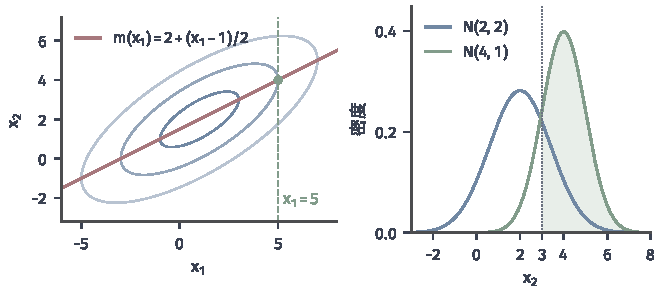
\includegraphics[width=112mm]{figures/01-basic-mathematics/05-probability-and-statistics-basics/matplotlib/rvec-gaussian-conditional/figure.pdf}
  \caption{二维高斯分布的条件化，参数为$\bm\mu=(1,2)^{\top}$、$\Sigma_{1,1}=4$、$\Sigma_{1,2}=2$、$\Sigma_{2,2}=2$。(a)蓝色椭圆是马氏距离为$1,2,3$的等密度线；红线是条件均值$m(x_1)=2+(x_1-1)/2$；绿色虚线标出观测$x_1=5$，圆点为该处的条件均值$4$。(b)蓝线是观测前$X_2$的边缘密度$\mathcal N(2,2)$，绿线是给定$X_1=5$后的条件密度$\mathcal N(4,1)$；阴影面积$\mathbb P(X_2>3\mid X_1=5)\approx0.84$。}
  \label{fig:rvec-gaussian-conditional}
\end{figure}

二维情形的公式可以用相关系数改写：$\mathbb E[X_2\mid X_1=x_1]=\mu_2+\rho\frac{\sigma_2}{\sigma_1}(x_1-\mu_1)$，$\operatorname{Var}(X_2\mid X_1=x_1)=\sigma_2^2(1-\rho^2)$。本例$\rho^2=1/2$，条件方差恰为边缘方差的一半；$|\rho|$越接近$1$，观测$X_1$后$X_2$的剩余不确定性越小。与示例~\ref{ex:rvec-study-table}中随$x$变化的条件方差相比，“条件方差不依赖观测值”是高斯模型的特殊性质。条件均值关于观测是一条直线，这也是第~\ref{sec:pred-regression}节简单线性回归模型的概率背景。

\FloatBarrier
\section{本章小结}
\label{sec:rvec-summary}

联合分布描述几个随机变量在同一次试验中的共同取值，可以用联合质量函数、联合密度或联合分布函数表示。边缘分布由联合分布求和或积分得到，但边缘相同的联合分布可以截然不同。均值向量描述共同的中心，协方差矩阵通过$\operatorname{Var}(\bm a^{\top}\bm X)=\bm a^{\top}\bm\Sigma\bm a$概括所有线性组合的波动；相关系数只度量线性关联，协方差矩阵奇异则对应以概率$1$成立的线性约束。

独立与条件分布从两个方向描述变量之间的信息。独立要求联合分布分解为边缘之积，它推出不相关，反之不成立；两两独立也推不出相互独立。条件分布由联合分布按观测值切片再归一化得到，全概率、全期望和全方差公式把条件层面的量汇总回总体。条件独立与无条件独立互不蕴含：共享的未知参数会让条件独立的观测在边缘上相关。

变换与生成是方向相反的两个问题。多元变量替换、卷积和辅助变量方法从已知分布计算组合量的分布，由此得到了二项分布、Gamma分布与Beta分布之间的联系；逆变换采样与按条件分解逐个生成，则从均匀输入出发构造目标分布，混合分布与层次模型都是条件生成的例子。

多元高斯分布把这些操作汇集在两个参数上：由独立标准高斯变量经$\bm\mu+\bm L\bm Z$生成，仿射变换后仍是高斯，边缘化只需取子向量与子矩阵，零交叉协方差即推出独立，条件分布的均值是观测的仿射函数、协方差是Schur补。本章始终假定分布已知；下一章转向相反的问题：只观察到数据时，怎样构造统计量并估计未知的分布参数（第~\ref{chap:sample-estimation}章）。
